%!TEX root = ../swiatlow_thesis.tex
\label{chapter:color}
\section{Introduction}


\section{Quark/Gluon Discrimination}
\label{jet-reconstruction:qg}
\subsection{Overview}
\label{jet-reconstruction:qg:overview}
%~\cite{Miyazawa:1966,Ramond:1971gb,Golfand:1971iw,Neveu:1971rx,Neveu:1971iv,Gervais:1971ji,Volkov:1973ix,Wess:1973kz,Wess:1974tw}

Just as $b$-tagging is useful for search for new physics in channels with heavy flavor, the identification of \textit{light quarks} can also be important when searching for new physics. Most commonly, the jets associated with multi-jet production arise from gluon radiation, and so a tool to eliminate these backgrounds can be very useful. Even searches for the Higgs boson decaying to hadronic $W$-bosons or $Z$-bosons can benefit, as once again the signal is dominated by light-quark jets and backgrounds are often gluon-induced.

This type of discrimination has been attempted at several experiments before ATLAS~\cite{TevatronShapes1,QGNN,Pumplin,QGopal,Ariel,QGsub,QGlep,QGcleo,DelphiQG,DelphiQG2,AlephQG,L3QG}. This discrimination tends to rely on the different color charges for quarks ($C_F=4/3$) and gluons ($C_A=3$), which leads to a leading order prediction that gluon jets have $C_A/C_F = 9/4$ more particles (which are consequently more widely distributed, and generally softer) than light-quark jets. OPAL's measurement~\cite{QGopal} indeed measured something very similar to this prediction. Because of their much simpler experimental environments, experiments like OPAL at $e^+/e^-$ colliders have generally been much more successful at discriminating between quarks and gluons, as determining ``pure'' samples at a hadron collider is exceedingly difficult. However, recent developments from the theory communited have suggested not just that pure samples suitable for calibration are obtainable, but also that discrimination is possible in the challenging underlying-event and pileup heavy environment of a hadron collider~\cite{schwartz1,schwartz2}. 

This section follows the results of the ATLAS paper on quark-gluon discrimination using 2011 data~\cite{ATLASqg,Golling:1554107}. First, quark and gluon jets are more precisely defined, followed by a description of possible discriminating variables. The use of data-driven templates is discussed, and such templates are validated in independent data samples. Finally, the tagger properties and power are presented, as well as scale-factors which can calibrate the MC to the observed performance in data. This work was done in collaboration with Larry Lee (then of Yale, now of University of Adelaide), David Lopez Mateos (Harvard University), and Zachary Marshall (then of CERN, now of Lawrence Berkeley National Laboratory).

\subsection{Definition of Light Quark and Gluon Jets}
\label{jet-reconstruction:qg:definition}

The labeling of a $b$-jet or a $c$-jet is a fairly straightforward process: the initiating $b$ and $c$ quarks, though unmeasurable and therefore un-physical themselves, inevitably hadronize into observable $B$ and $D$ hadrons. Thus, the presence of a $B$ or $D$ hadron, at the MC simulation level, is enough to provide a label to the jet: if a $B$ or $D$ hadron is present, it is clear that a secondary vertex can occur, and the jet should be counted as being heavy-flavor.

This unambiguous hadronization does not occur for light-quark and gluon jets. In the parton shower process, gluons even split into pairs of quarks before hadronization: all gluon jets contain quarks, in this sense. Moreover, the observable particles--- kaons, pions, protons, neutrons, and so on--- are all identical for quark and gluon initiated jets. Even before attempting discrimination between the two classes, then, it is difficult to precisely state what we are discriminating between.

One potentially less ambiguous definition is to use the partons from the matrix element to label jets. This has the disadvantage that only some jets can be labelled--- in particular, in multi-jet events, depending on the generator, as few as 2 partons are simulated as part of the matrix element, and therefore only two jets out of many could be labelled. A better strategy is to simply use the highest energy parton within $\Delta R < R_\mathrm{jet}$ of the jet. When studied with both \Pythia $2\rightarrow2$ and MadGraph $2\rightarrow4$ generators, this matching followed the labelling from the matrix element in $> 95\%$ of events. This labelling has the advantage of also working on the hadronic decays of top quarks or $Z$-bosons. For the rest of the discussions in this section, this labeling scheme will be implied when discussing quark and gluon jets.

While this analysis does not directly attempt to tag $b$ and $c$ jets, they must often be subtracted from the samples in order to deal with only light-flavor jets. These jets are labelled with the following priority: if a $B$-hadron with $\pt > 5$ GeV exists within $\Delta R < R_\mathrm{jet}$, label it a $b$-jet. If two such independent hadrons exist, label it a $bb$ jet (originating from a gluon splitting, but not considered in this analysis as the heavy-flavor component shapes the jet more than the gluon origin). If this fails, search for a $D$-hadron with $\pt > 5$ GeV within the jet; if one is found, label it a $c$-jet, and if two are found, label it $cc$. Only after these steps have determined that there are no heavy flavor quarks within the jet is the jet's light-flavor type assessed.

\subsection{Data and MC Samples}
\label{jet-reconstruction:qg:samples}

Several different data and MC samples are used to study the properties of quark and gluon jets. There are two main categories: multi-jet and $\gamma$+jet events. 

Multi-jet events are modelled by {\sc Pythia 6} and \Herwig++ simulation, and some smaller samples using {\sc Madgraph} interfaced with {\sc Pythia 8}. Events are selected in data with single jet triggers with various thresholds which are fully efficient at $\pt > 40$~GeV. The lower \pt threshhold triggers are \textit{prescaled} to reduce the rate at high luminosity. When binning results in \pt, each bin is filled exclusively with events from a single trigger that is fully efficient in that range (and the second jet is used only if its \pt also is in this same bin). When studying tri-jet events, the same \pt binning and trigger treshholds are used.

The $\gamma$+jet sample is selected with single photon triggers, again with variable tresholds and corresponding prescales. The lowest threshold is at $p_\mathrm{T}^\gamma > 25$~GeV, and a back-to-back requirement between the $\gamma$ and jet, $\Delta \phi > 2.8$, is imposed. An additional veto on soft radiation is imposed, wherein the uncalibrated \pt of the sub-leading jet is required to be less than $30\%$ of $p_\mathrm{T}^\gamma$~\cite{JES2010}\footnote{In the corresponding 2012 analysis, it was discovered that this cut changes the \pt distribution within each \pt bin and slightly biases the result, lowering slightly the performance of the tagger.}. Each jet \pt bin is filled by a single-photon trigger that is fully efficient in that bin, as the balance between photon and jet guarantees. The same triggers are used in the $\gamma$+2jet sample, except that the subleading jet \pt cut is removed.

% The dijet sample is selected using single-jet triggers with various thresholds [48], which are fully efficient for jets with pT > 40 GeV. Each jet pT bin is filled exclusively by a single trigger that is fully efficient for jets in that pT range, following Ref. [1]. The trijet sample uses the same trigger selection as the dijet sample. This guarantees that studies using the jet with the third highest pT in each event are not biased by the trigger.

%The γ+jet sample is selected using single-photon trig-gers. The lowest threshold single-photon trigger is fully efficient for photons with pT > 25 GeV. For this sam- ple, a back-to-back requirement for the photon and the leading jet, ∆φ > 2.8, is imposed. An additional veto on soft radiation is also applied to further reduce back- ground contamination [41]: the uncalibrated pT of the sub-leading jet is required to be less than 30% of the photon pT. Relying on the pT balance of the photon and jet, each jet pT bin is filled exclusively by a single-photon trigger that provides a fully efficient selection.
%The same triggers are used in the γ+2-jet sample in each region of jet pT. Since the sub-leading jet pT is lower than that of the leading jet by definition, this selection is also not biased by jet reconstruction effects.

\subsection{Quark and Gluon Jet Properties}
\label{jet-reconstruction:qg:properties}

Given the expectations developed in Section~\ref{jet-reconstruction:qg:overview}, there are many different jet observables which could potentially distinguish between quark and gluon initiated jets. One approach is to try to measure the number of particles to take advantage of the color factor difference. In principle, a variable just as $n_\mathrm{clusters}$ would be ideal, as it is expected to be directly proportional to the number of stable particles interacting with the calorimeter. However, as the granularity of the calorimeter changes with $\eta$, and the number of clusters grows unbounded with pileup, this is not a very useful variable. A related alternative is \ntrk, the number of tracks associated to a jet\footnote{Note that in this analysis, tracks are associated with a $\Delta R < R_\mathrm{jet}$ requirement instead of a ghost association as defined in Section~\ref{jet-reconstruction:pileup:ghost-association}. As most jets considered are isolated, and \antikt~is used throughout, this is a reasonable simplification.}. This is expected to have much less $\eta$ dependence, and because tracks from pileup vertices are able to be rejected, is stable with regards to the amount of pileup.

Other variables take into account the radial distribution of the energy inside the jet. One simple such variable is the \textit{jet width}, as discussed in Section~\ref{jet-reconstruction:calibration:gsc}. The width is the first radial moment of the \pt of the jet: jets with a very focused core will have lower width, and jets with a more even distribution of energy will have a higher width. Gluons, because they first split to quarks, and because of their higher color factor, are expected to have broader energy distributions and therefore higher width. The width can be calculated with clusters as inputs, or the tracks associated to a jet. Because of the issues with pileup (which are expected to change the distribution of the width as a function of the number of interactions, if the variable is calculated with calorimeter inputs), track width is used in this analysis.

Many other variables, as documented in \cite{schwartz1}, are possible, but these two were the preferred combination from early theoretical studies. Another set of studies~\cite{EEC} indicated that a new observable, the energy-energy correlated angularity, could also be useful. This class of observables is defined as:
\begin{equation}
{\rm ang_{\rm EEC}}=\frac{ \sum_i \sum_j p_{{\rm T},i} \times p_{{\rm T},j} \times (\Delta R(i,j))^\beta}{ (\sum_i p_{{\rm T},i})^2 },
\end{equation}
where $i$ runs over the tracks associated to the jet and $j$ runs over the tracks associated to the jet with $j>i$ (the calorimeter version is sensitive to pileup, and therefore not studied), and $\beta$ is a tunable parameter typically $O(1)$. While this variable is in principle very sensitive, several effects conspire to limit its effectiveness and prevent it from being used in the final result (and will be discussed shortly).

To characterize the separation between quark and gluon jets with these variables, we define the \textit{separation} as~\cite{2006physics11219P}:
%
\begin{equation}
s=\frac{1}{2}\int\frac{(p_q(x)-p_g(x))^2}{p_q(x)+p_g(x)}dx = \frac{1}{2}\sum_i\frac{(p_{q,i}-p_{g,i})^2}{p_{q,i}+p_{g,i}}, 
\label{eq:separation}
\end{equation}
%
where $i$ runs over bins of a histogram. This is a measure of the overlap of two distributions, $q(x)$ and $g(x)$, which are the quark and gluon distributions respectively in a Pythia dijet simulation.  The result is shown in Figure~\ref{fig:jet-reconstruction:qg:separation}: in general, the separation power increases as a function of \pt, and \ntrk is predicted to have the best power. Track width performs worse than many of the other variables, but because of its resilience in modeling (compared to the EEC variables) and its robustness to pileup (compared to the calorimeter width), it will also be studied further. Moreover, the track width has a very low correlation with \ntrk: as low as $15\%$ at low \pt and only $50\%$ at high \pt, whereas the EEC variables have consistent correlations of $75\%$. This means that a combined observable from \ntrk and track width will likely outperform other options.

%%%%%%%%%%%%%%%%

\begin{figure}
\centering
\includegraphics[width=0.6\textwidth]{qg/SeparationPower}
\label{fig:jet-reconstruction:qg:separation}
\caption{The size of the scale factor for $b$-tagging calibration in data, as a function of the jet \pt, and the size of the corresponding uncertainties.}
\end{figure}

%%%%%%%%%%%%%%%% 

\subsection{Data-Driven Templates}

Figures~\ref{fig:jet-reconstruction:qg:dijetProperties} and \ref{fig:jet-reconstruction:qg:gammajetProperties} show the \ntrk and Track Width distributions for data, \Pythia, and \Herwigpp generators, in both dijet and $\gamma$+jet topologies, at low \pt and high \pt. The distributions show that while there is decent agreement for the width, the \ntrk variable is very poorly modelled: \Pythia predicts too many tracks consistently, while \Herwigpp predicts too few. 

\begin{figure}[tbp]
\begin{center}
\subfigure[]{
\includegraphics[width=0.48\textwidth]{qg/dijetakt4TopoEM_ntrk_PT60_eta0.pdf}
}
\subfigure[]{
\includegraphics[width=0.48\textwidth]{qg/dijetakt4TopoEM_ntrk_PT260_eta0.pdf}
} \\
\subfigure[]{
\includegraphics[width=0.48\textwidth]{qg/dijetakt4TopoEM_trkwidth_PT60_eta0.pdf}
}
\subfigure[]{
\includegraphics[width=0.48\textwidth]{qg/dijetakt4TopoEM_trkwidth_PT260_eta0.pdf}
}
\caption{
Jet \ntrk (top) and track width (bottom) for jets with $60<\pt<80$~\GeV\ (left) and
$260<\pt<310$~\GeV\ (right) in {\sc Pythia} 6, {\sc Herwig++}, and data, for a dijet selection.
Jets have $|\eta|<0.8$ and are reconstructed with an \AKT\ jet algorithm with $R=0.4$.
 }
\label{fig:jet-reconstruction:qg:dijetProperties}
\end{center}
\end{figure}

\begin{figure}[tbp]
\begin{center}
\subfigure[]{
\includegraphics[width=0.48\textwidth]{qg/gammaakt4TopoEM_ntrk_PT60_eta0.pdf}
}
\subfigure[]{
\includegraphics[width=0.48\textwidth]{qg/gammaakt4TopoEM_ntrk_PT260_eta0.pdf}
} \\
\subfigure[]{
\includegraphics[width=0.48\textwidth]{qg/gammaakt4TopoEM_trkwidth_PT60_eta0.pdf}
}
\subfigure[]{
\includegraphics[width=0.48\textwidth]{qg/gammaakt4TopoEM_trkwidth_PT260_eta0.pdf}
}
\caption{
Jet \ntrk (top) and track width (bottom) for jets with $60<\pt<80$~\GeV\ (left) and
$260<\pt<310$~\GeV\ (right) in {\sc Pythia} 6, {\sc Herwig++}, and data, for a $\gamma+$jet selection.
Jets have $|\eta|<0.8$ and are reconstructed with an \AKT\ jet algorithm with $R=0.4$.
 }
\label{fig:jet-reconstruction:qg:gammajetProperties}
\end{center}
\end{figure}

This makes the usual prospect of constructing a tagger--- beginning with a likelihood trained in MC and calibrating small residual differences in data--- a challenging prospect. Instead, we first extract a pure quark or gluon shape from data, and construct the tagger from these shapes. To construct these shapes, we look at histograms in two different samples, where we can measure the quark/gluon flavor fraction very precisely using the matrix element of the generator\footnote{And while generator hadronization properties vary greatly, this fraction of quark and gluon jets is rather consistent; any residual difference, at the $10\%$ level, is taken as a systematic later in the procedure.}. For each bin $i$ of jet $\eta$, jet $\pt$, and jet property (track width, number of tracks, or the two-dimensional distribution of the these), a set of linear equations is solved:
%
\begin{align}
P_i(\eta,\pt) &= f_{q}(\eta,\pt) \times P_{q,i}(\eta,\pt) \nonumber \\
	& + f_{g}(\eta,\pt) \times P_{g,i}(\eta,\pt) \nonumber \\
& + f_{c}(\eta,\pt) \times P_{c,i}(\eta,\pt) \nonumber \\
& + f_{b}(\eta,\pt) \times P_{b,i}(\eta,\pt) , 
\label{eq:fractions}
\end{align}
%
where $P_i$ is the value of the relevant distribution in bin $i$ of the distribution in the dijet
or $\gamma+$jet sample, $f_{q}$ and $f_{g}$ are the light-quark and gluon fractions 
predicted by \Pythia at a given $\eta$ and $\pt$, 
and $P_{q,i}$ and $P_{g,i}$ are the values of the relevant distribution 
for quark- and gluon-jets in bin $i$ of the distribution. The fractions 
$f_{c}$ and $f_{b}$ for $c$-jets and $b$-jets are relatively small. They are taken from the
MC simulation, together with the corresponding distributions $P_{c}$ and $P_{b}$.
The same is true for the fractions and distributions for $g\rightarrow c\bar{c}$ and $g\rightarrow b\bar{b}$,
not shown in Eq.~\ref{eq:fractions} for brevity. The heavy flavor fractions are typically below $5-10\%$, and are directly subtracted from the distributions.

This leaves two equations (one for a dijet sample, and one for $\gamma$+jet), with two unknowns ($P_{q}$ and $P_{g}$), which can be solved bin-by-bin. The only MC input is from the fractions, and the rest of the shape of the resulting distribution comes from data. The studies are performed in three bins of $|\eta|$: $|\eta|<0.8$, $0.8<|\eta|<1.2$ and $1.2<|\eta|<2.1$, though in general only the results from the central bin will be shown for the sake of brevity. Note that this technique depends on the assumption that the shape of a quark jet in a $\gamma$+jet sample is the same as that of a quark jet in a dijet sample: as we will later see, this is largely true, but residual differences will account for the largest systematic. An additional fake term,  $f_{{\rm fake}, i}(\eta,\pt)\times P_{{\rm fake}, i}(\eta,\pt)$, is added to the distributions in the $\gamma$+jet sample to take into account the fake photons which contaminate this sample~\cite{JES2011}.

This method is first tested for the individual distributions of \ntrk and Track Width in MC, as in the top subfigures of Figure~\ref{fig:jet-reconstruction:qg:ntrkWidthClos}. The closure in \Pythia is very good: the small residual differences between the extracted templates and the inputs are taken as a systematic later. The dijet sample, as it contains more gluons, is in some sense the basis of the gluon distribution; likewise, as the $\gamma$ is more likely to radiate from a charged object than a neutral, the $\gamma$+jet sample is more quark-enriched and the extraction leads to a quarks following the $\gamma$+jet sample more closely. With the technique validated in MC, we can also use it in data, replacing the relevant value from data into the $P_i$ of Equation~\ref{eq:fractions}. The results of this are shown in Figure~\ref{fig:jet-reconstruction:qg:ntrkWidthClos} in the bottom panel: we see now a confirmation of the earlier studies, in that the \ntrk variable is clearly poorly modelled by the MC. In particular, the \textit{gluon} distribution is strongly incorrect for \ntrk, while quarks fare better; the Track Width distribution is reasonably well modelled for both quarks and gluons, as expected. As the differences between data and MC make quarks and gluons more similar than predicted by the simulation, we can expect a degraded tagger performance compared to the naive expectation.


\begin{figure*}[p]
\begin{center}
%Subfigures
\subfigure[]{
\includegraphics[width=0.45\textwidth]{qg/ntrk_akt4TopoEM_eta0_means_withMCin_FromMC_Pyth}
}
\subfigure[]{
\includegraphics[width=0.45\textwidth]{qg/trkwidth_akt4TopoEM_eta0_means_withMCin_FromMC_Pyth}
} \\
\subfigure[]{
\includegraphics[width=0.45\textwidth]{qg/ntrk_akt4TopoEM_eta0_means_withMCin}
}
\subfigure[]{
\includegraphics[width=0.45\textwidth]{qg/trkwidth_akt4TopoEM_eta0_means_withMCin}
}
\caption{ Average (a,c) \ntrk and (b,d) track width for quark- (solid symbols) and gluon-jets
(open symbols) as a function of reconstructed jet $\pt$ for isolated jets with $|\eta|<0.8$.
Results are shown for distributions obtained using the template extraction method in
\Pythia 6 simulation (black circles, (a,b)) or data (black circles, (c,d)), as well as for 
labeled jets in the dijet sample (triangles) and in the $\gamma$+jet sample (squares).
The error bars represent only statistical uncertainties. Isolated jets are reconstructed using the
\akt jet algorithm with radius parameter $R=0.4$. The bottom panels show
the ratio of the results obtained with the in-situ extraction method to the results
in the dijet and $\gamma$+jet MC samples. }
\label{fig:jet-reconstruction:qg:ntrkWidthClos}
\end{center}
\end{figure*}

There are several sources of uncertainty in the extraction procedure:

\begin{enumerate}
\item Uncertainties on input fractions ($f_{x,i}$)
\item Uncertainties on the input shapes ($P_{x,i}$) 
\item Uncertainties on the fake photon background
\item Sample dependent effects (the differences between quarks in $\gamma$+jet and dijet samples)
\end{enumerate}

The input fraction uncertainties are addressed by comparing the fractions in \Pythia and {\sc Madgraph}, and taking the difference as directly as a systematic. This takes into account differences potentially due to different renormalization/factorization scales, and the different ways of simulating the emission of quarks/gluons. A $5\%$ uncertainty, anti-correlated between the quark and gluon fractions, is assigned as a conservative systematic. The differences due to the mismodelling of the PDF is also included as a systematic. A combination of different PDF sets are assessed, each with different properties. They use different fitting procedures (MRST, CTEQ, and NNPDF), and are accurate to different orders in the perturabtive expansion (MSTW2008lo for LO, CT10 for NLO), and have different assumptions about the $\alpha_s$ calculation (MRST2007lmod for LO$^*$ and MRSTMCal for LO$^{**}$). Another $5\%$ anti-correlated systematic takes these effects into account conservatively.

Uncertainties on the shapes come from the MC dependence on the $b$ and $c$-jet shapes. Uncertainties on the $b$-jet shapes are determined from a $t\bar{t}$ sample with $> 95\%$ purity: a $10\%$ systematic is assigned on the $b$-jet properties to take this into account~\cite{Golling:1554107}. For $c$-jets, templates with 10\% increases in the rates of 2-prong, 3-prong, and 4-prong decays are used to estimate the effect of changes to the $c$-hadron decay~\cite{Golling:1554107}. The largest propagated difference of these is used as the systematic uncertainty on the tagger.

The fake photon background is assessed in several ways. The fake-factors are developed using an ABCD procedure, and the cuts used to define each of the regions are varied to assess the sensitivity to these effects~\cite{JES2011}. This results in a purity difference of $10\%$ for low \pt jets, and is the dominant uncertainty related to the photon measurement.

The sample dependent uncertainty is the largest, and takes into account the differences in the MC's seen in Figure~\ref{fig:jet-reconstruction:qg:ntrkWidthClos}. 
Uncertainties on the jet properties are estimated first from differences
between the $\gamma+$jet and dijet samples of the properties of quark- and gluon-jets, using both \Pythia and \Herwigpp. The envelope of these
variations is used to estimate a systematic uncertainty, but is prone to large fluctuations due to the limited statistics of the MC samples. These statistical 
uncertainties
are estimated and used to smooth the $\pt$ dependence of the uncertainty following the
procedure described in \cite{JES2011}: a Gaussian kernel with size proportional to the inverse of the uncertainty averages over the \pt bins, weighting those with lower statistical uncertainty higher. 
The sample dependence is consistently the dominant systematic uncertainty for all jet $\pt$, and thus it is critical to take into account these variations.

\subsection{Validation with event-level kinematic cuts}
\label{jet-reconstruction:qg:validation}

While the shapes derived in the previous section are data-driven, the large data and MC differences motivate an independent check in completely separate samples for the purpose of validation. Luckily, \cite{schwartz2} proposed several samples, accessible at hadron colliders, with quark/gluon purity of $> 90\%$ which could be used for validation purposes. These samples are very statistically limited and therefore insufficient to determine the shapes used for a tagger themselves, but can serve very well as test samples. Moreover, these independent samples give a feeling for any residual color-flow or event-level dependence which the previous uncertainty procedure may have missed.

Gluon jets are found in the dijet sample, particularly because the proton have a very large gluon component at low $x$. However, as \pt rises, the gluon fraction falls off rapidly, leaving a mixed sample when measured at any appreciable \pt. In multi-jet events, however, any radiated jet is relatively more likely to originate from a gluon. As this radiation is likely to be soft, the third-leading jet is thus more likely to be a gluon. A kinematic discriminant, using only information on the relative location of jets, can further purify the tri-jet sample: 
%
\begin{equation}
\zeta=|\eta_3|-|\eta_1-\eta_2|,
\end{equation}
%
where $\eta_i$ is the pseudorapidity of the $i$th leading jet. Cutting on $\zeta < 0$ results in a tri-jet sample with gluon purity $> 90\%$, as determined in {\sc Madgraph} simulation. To evaluate the determination of the gluon shapes from Figure~\ref{fig:jet-reconstruction:qg:ntrkWidthClos}, those templates are directly compared to the sample with $\zeta < 0$. This comparison is presented in \ref{fig:jet-reconstruction:qg:pure_trijet_ntrkTrkWidth1} and \ref{fig:jet-reconstruction:qg:pure_trijet_ntrkTrkWidth2} of Figure~\ref{fig:jet-reconstruction:qg:pure_trijet_ntrkTrkWidth}. The agreement between the extracted template and the completely independent pure data sample of gluons is very good, for both \ntrk and Track Width. In particular, the \ntrk distributions agree quite well, and the purified sample agrees better with the data than the \Pythia simulation.

\begin{figure}[p]
\begin{center}
\subfigure[]{
\label{fig:jet-reconstruction:qg:pure_trijet_ntrkTrkWidth1}
\includegraphics[width=0.45\textwidth]{/qg/smoothed_ntrk_akt4TopoEM_eta0_PureExtractedG}
}
\subfigure[]{
\label{fig:jet-reconstruction:qg:pure_trijet_ntrkTrkWidth2}
\includegraphics[width=0.45\textwidth]{qg/smoothed_trkwidth_akt4TopoEM_eta0_PureExtractedG}
} \\
\subfigure[]{
\label{fig:jet-reconstruction:qg:pure_trijet_ntrkTrkWidth3}
\includegraphics[width=0.45\textwidth]{qg/smoothed_ntrk_akt4TopoEM_eta0_PureExtractedQ}
}
\subfigure[]{
\label{fig:jet-reconstruction:qg:pure_trijet_ntrkTrkWidth4}
\includegraphics[width=0.45\textwidth]{qg/smoothed_trkwidth_akt4TopoEM_eta0_PureExtractedQ}
}
\caption{Top, the jet (a) \ntrk and (b) track width as a function of $\pt$ for jets in a
gluon-jet-enriched trijet sample (triangles) compared to gluon-jet extracted templates (circles) for
$|\eta|<0.8$. Bottom, the jet (c) \ntrk and (d) track width as a function of $\pt$ for jets in a quark-jet-enriched $\gamma$+jet
sample (triangles) compared to quark-jet extracted templates (circles) for jets with $|\eta|<0.8$.
Jets are reconstructed with the \antikt algorithm with $R=0.4$. The bottom
panels of the figures show the ratios of the results found in the enriched sample to the extracted
results. Error bars on
the points for the enriched sample correspond to statistical uncertainties. The inner
shaded band around the circles and in the ratio represents statistical uncertainties on the
extracted results, while the outer error band represents the combined systematic and statistical
uncertainties.
}
\label{fig:jet-reconstruction:qg:pure_trijet_ntrkTrkWidth}
\end{center}
\end{figure}

Events with photons are already used to extract the more quark-like component of the templates: events with one jet and one photon have $>80\%$ quark purity at $\pt > 150$~GeV. Enrichment of this sample is difficult, and anyway, we have already used it for the template extraction and so validation requires a new sample. A sample with a single photon and two jets turns out to be more effective~\cite{schwartz2}: if no additional selection is applied, they have a lower purity, but another kinematic event-level cut can be used to significantly purify the sample by helping to identify the jets seeded by the parton that is most likely to have radiated the photon (which is more likely to be a quark because the photon requires electric charge to be radiated). The observable is defined as:
%
\begin{equation}
\xi=\eta_\text{jet~1}\times\eta_\gamma+\Delta R_{(\text{jet~2},\gamma)},
\end{equation}
%
where $\eta_\gamma$ ($\eta_\text{jet~1}$) is the $\eta$ of the photon (leading jet), and 
$\Delta R_{(\text{jet~2},\gamma)}$ gives the difference in $\eta$--$\phi$ space between the sub-leading 
jet and the photon. By imposing a requirement on this variable of $\xi < 1$, purities over 90\% can be achieved (as validated with {\sc Madgraph} siulation), although with a significant loss of events. This sample can again be compared to the extracted templates for quarks from Figure~\ref{fig:jet-reconstruction:qg:ntrkWidthClos}. This comparison is presented in \ref{fig:jet-reconstruction:qg:pure_trijet_ntrkTrkWidth3} and \ref{fig:jet-reconstruction:qg:pure_trijet_ntrkTrkWidth4} of Figure~\ref{fig:jet-reconstruction:qg:pure_trijet_ntrkTrkWidth}. Once again, the agreement between the independent data sample and the extracted templates is very good for both the \ntrk and Track Width variables, validating our use of our templates for both quark and gluon jets.

\subsection{Creating a Tagger, and Results}

As the discriminating power of Track Width and \ntrk changes with \pt (\ntrk gains power as \pt rises, while the opposite is true for Track Width), a combined likelihood between the two variables will be the most effective tool for quark-jet tagging\footnote{Though a gluon jet tagger is also possible, the details are not considered in this analysis.}. Such a likelihood is defined using the normalized extracted two-dimensional distributions (called $q$ and $g$),
%
\begin{equation}
L=\frac{q}{q+g}.
\end{equation}
%
A cut on this variable $L$, built in bins of \pt and $\eta$, will effectively discriminate between quarks and gluons. Note that the two-dimensional distributions are first smoothed with a Gaussian kernel and dynamically rebinned to ensure that all regions of the distributions are populated sufficiently\footnote{In particular, low statistics in the $q$ distribution also causes a rebinning of the $g$ distribution, in order to make the likelihood construction as simple as possible. To rebinning covers only areas of the distribution which are statistically limited: regions sufficiently populated are not rebinned}. The two-dimensional distribution of $L$ is shown in the top of Figure~\ref{fig:jet-reconstruction:qg:likelihoodSample}, for both data and MC: it is clear that the taggers have very different properties in data and in the simulation. This figure also contains the projections of the $L$ variable, when using the quark and gluon distributions used to build the tagger, before smoothing. Separation clearly exists for both data and MC taggers, but is much stronger in MC.



\begin{figure}[tbp]
\begin{center}
\subfigure[]{
\includegraphics[width=0.48\textwidth]{qg/width_vs_ntrk_PT160_akt4TopoEM_eta0_2dT_llhood_q_.pdf}
}
\subfigure[]{
\includegraphics[width=0.48\textwidth]{qg/width_vs_ntrk_PT160_akt4TopoEM_eta0_2dT_llhood_q__FromMC.pdf}
}
\subfigure[]{
\includegraphics[width=0.48\textwidth]{qg/width_vs_ntrk_PT160_akt4TopoEM_eta0_oneDim_q_.pdf}
}
\subfigure[]{
\includegraphics[width=0.48\textwidth]{qg/width_vs_ntrk_PT160_akt4TopoEM_eta0_oneDim_q__FromMC.pdf}
}
\caption{ Value of the likelihood-based ratio $L$ as a function of \ntrk and track width (top) and 
likelihood-based discriminant distribution for quark- and gluon-jets (bottom) for isolated jets 
of $|\eta|<0.8$ and $160<\pt<210\GeV$. The plots have been obtained using data (left) and
a \Pythia 6 dijet sample (right). Jets are reconstructed using the \akt\ jet algorithm
with radius parameter $R=0.4$. }
\label{fig:jet-reconstruction:qg:likelihoodSample}
\end{center}
\end{figure}

The performance of the tagger is determined using the two dimensional templates extracted from data, before smoothing, and for labelled jets in MC simulations. The tagger is independently derived in \Pythia and \Herwigpp, following the same procedure as in data. Systematic uncertainties are estimated by deriving alternative templates as described in the previous section and determining the change in efficiency and rejection for the same cut on $L$. Table~\ref{tab:perfSummary} summarizes this performance for jets with $|\eta|<0.8$. Several different operating points, at $30\%$, $50\%$, $70\%$, and $90\%$ quark efficiency are evaluated. The statistical uncertainty is determined using pseudoexperiments via bootstrapping. Systematic uncertainties are combined in quadrature. Scale factors between data and MC are computed for the gluon efficiencies: quark efficiencies by definition have a scale factor of 1 (though there is some uncertainty) as the tagger (and the associated cut) is derived separately in data and MC. Several different \pt bins are shown in the table. 


\begin{table}[htbp]
\caption{
Summary of the performance of the quark-jet tagger on quark- and gluon-jets in data and \Pythia MC simulation for jets built with the \antikt algorithm with $R=0.4$ and with $|\eta|<0.8$. 
The first error corresponds to the statistical uncertainty, while the second corresponds to the systematic uncertainty.
The scale factor is the ratio of data to MC simulation. 
\label{tab:perfSummary}}
\begin{center}
\begin{tabular}{|c|l|l|l|l|l|l|}
\hline
& \multicolumn{2}{|c|}{Monte Carlo} & \multicolumn{2}{|c|}{Data} & \multicolumn{2}{|c|}{Scale Factor} \\ 
\hline
& $\epsilon_{\rm quark}$ & $\epsilon_{\rm gluon}$ & $\epsilon_{\rm quark}$ & $\epsilon_{\rm gluon}$ & SF$_{\rm quark}$ & SF$_{\rm gluon}$ \\
\hline\noalign{\smallskip}
\multirow{4}{*}{\begin{sideways}$\pt=60$--$80 \GeV$\end{sideways}} 
& 30\% &  8.4\% &  ($30.0\pm0.8^{+3.2}_{-5.3}$)\%    &  ($11.9\pm0.3^{+7.5}_{-2.9}$)\%    &  $1.00\pm0.03^{+0.11}_{-0.18}$ & $1.42\pm0.04^{+0.89}_{-0.34}$ \\&&&&&&\\
& 50\% & 21.0\% &  ($50.0^{+1.4+4.3}_{-1.3-6.8}$)\%  &  ($26.6^{+0.8+7.1}_{-0.6-3.9}$)\%  &  $1.00^{+0.027+0.09}_{-0.026-0.14}$ & $1.27^{+0.04+0.34}_{-0.03-0.19}$ \\&&&&&&\\
& 70\% & 41.5\% &  ($70.0^{+1.7+3.9}_{-1.5-11.0}$)\%  &  ($48.4^{+1.1+4.7}_{-0.9-6.0}$)\%  &  $1.00^{+0.024+0.06}_{-0.022-0.16}$ & $1.17^{+0.03+0.11}_{-0.02-0.14}$ \\&&&&&&\\
& 90\% & 69.9\% &  ($90.0^{+1.5+1.7}_{-1.3-3.3}$)\%  &  ($80.2^{+1.0+5.6}_{-0.8-2.2}$)\%   &  $1.00^{+0.02+0.02}_{-0.01-0.04}$ & $1.15^{+0.015+0.08}_{-0.012-0.03}$ \\&&&&&&\\
\hline\noalign{\smallskip}
\multirow{4}{*}{\begin{sideways}\centering$\pt=110$--$160 \GeV$\end{sideways}} 
& 30\% &  5.7\% &  ($30.0\pm0.6^{+2.8}_{-4.6}$)\%  & ($11.6^{+0.6+6.2}_{-0.4-4.6}$)\%   & $1.00\pm0.02^{+0.09}_{-0.15}$ & $2.03^{+0.11+1.08}_{-0.08-0.81}$ \\ &&&&&&\\
& 50\% & 13.9\% &  ($50.0\pm1.0^{+4.1}_{-6.1}$)\%  & ($24.3^{+1.2+7.4}_{-0.8-9.2}$)\%   & $1.00\pm0.02^{+0.08}_{-0.12}$ & $1.75^{+0.09+0.53}_{-0.06-0.66}$ \\ &&&&&&\\
& 70\% & 29.7\% &  ($70.0^{+1.0+3.9}_{-1.1-8.5}$)\%  & ($45.3^{+1.5+4.6}_{-1.1-9.3}$)\% & $1.00^{+0.01+0.06}_{-0.02-0.12}$ & $1.52^{+0.05+0.15}_{-0.04-0.31}$ \\ &&&&&&\\
& 90\% & 64.8\% &  ($90.0^{+0.5+2.0}_{-0.6-2.6}$)\%  & ($78.1^{+1.0+3.5}_{-0.6-6.0}$)\% & $1.00^{+0.006+0.02}_{-0.007-0.03}$ & $1.21^{+0.02+0.05}_{-0.01-0.09}$ \\ &&&&&&\\
\hline\noalign{\smallskip}
\multirow{4}{*}{\begin{sideways}\centering$\pt=310$--$360 \GeV$\end{sideways}} 
& 30\% &  3.9\% & ($30.0^{+5.0+2.1}_{-7.1-4.7}$)\% & ($11^{+5+8}_{-7-4}$)\% & $1.00^{+0.17+0.07}_{-0.24-0.16}$ & $2.8^{+1.4+2.0}_{-1.9-1.1}$ \\&&&&&&\\
& 50\% & 10.3\% & ($50.0^{+8.1+3.0}_{-11.6-8.3}$)\%& ($23^{+10+8}_{-12-9}$)\%& $1.00^{+0.16+0.06}_{-0.23-0.17}$ & $2.2^{+1.0+0.8}_{-1.1-0.9}$ \\&&&&&&\\
& 70\% & 23.5\% & ($70.0^{+7.2+3.1}_{-8.8-7.0}$)\% & ($43^{+8+6}_{-12-10}$)\% & $1.00^{+0.10+0.04}_{-0.13-0.10}$ & $1.81^{+0.35+0.23}_{-0.51-0.42}$ \\&&&&&&\\
& 90\% & 58.9\% & ($90.0^{+5.0+1.8}_{-4.9-3.1}$)\% & ($80^{+6+4}_{-10-7}$)\% & $1.00^{+0.06+0.02}_{-0.05-0.03}$ & $1.37^{+0.10+0.07}_{-0.17-0.11}$ \\&&&&&&\\
%\vspace[-0.1]
\hline
\end{tabular}
\end{center}
\end{table}

The largest scale factors occur at high \pt for the tightest operating point, where the difference between the predicted and observed \ntrk distributions are largest. Looser operating points, and lower \pt, have lower scale factors. Interestingly, the efficiency in data changes much less with \pt than predicted by \Pythia: the simulation seems to predict the strongly growing strength of \ntrk with \pt, while the true gain is much slower. Results are shown only for the central $\eta$ bin, but are consistent across $\eta$ (though uncertainties, especially statistical, are higher at higher $\eta$).

Figure~\ref{fig:jet-reconstruction:qg:perf_summary} shows a summary of the performance, by plotting the quark efficiency vs the gluon efficiency in data and several simulations, for two different \pt bins. \Pythia clearly shows a significantly lower gluon efficiency, i.e. an over-performance of the tagger. \Herwigpp shows a slightly higher gluon efficiency than in data, i.e. an under-performance of the tagger, though it is not significant outside of the uncertainties for some of the \pt bins and operating points.

\begin{figure}[!htp]
\begin{center}
\subfigure[]{
\includegraphics[width=0.45\textwidth]{qg/smoothed_akt4TopoEM_eta0_PT60_EffcienciesVsQEffHerwig.pdf}
\label{fig:jet-reconstruction:qg:perf_summary_a}
}
\subfigure[]{
\includegraphics[width=0.45\textwidth]{qg/smoothed_akt4TopoEM_eta0_PT210_EffcienciesVsQEffHerwig.pdf}
\label{fig:jet-reconstruction:qg:perf_summary_b}
}
\caption{ Gluon-jet efficiency as a function of quark-jet efficiency calculated using jet 
properties extracted from data (solid symbols) and from MC-labeled jets
from the dijet \Pythia (empty squares) and \Herwigpp (empty diamonds) samples. 
Jets with (a) $60<\pt<80$~\GeV\ and (b) $210<\pt<260$~\GeV\  and $|\eta|<0.8$
are reconstructed with the anti-$k_t$ algorithm with $R=0.4$.
The shaded band shows the total systematic uncertainty on the data. The bottom of the plot
shows the ratios of each MC simulation to the data. The error bands on the performance
in the data are drawn around 1.0. 
}
\label{fig:jet-reconstruction:qg:perf_summary}
\end{center}
\end{figure}

The performance of the tagger can also be measured usign the purified samples, i.e. the tri-jet and $\gamma$+2jet samples. The results of these comparisons are shown in Figure~\ref{fig:jet-reconstruction:qg:perf_summary_pur}, at low \pt and high \pt. The performance in the purified sample is very similar to the data samples used to train the tagger, though the results are statistically limited. In any case, the tagging performance may be slightly worse in these samples, and is again not near the prediction from \Pythia. Figure~\ref{fig:jet-reconstruction:qg:perfDataMC} shows the performance, separately for each operating point, as a function of the jet \pt, in \Pythia, the nominal extracted data samples, and the purified data samples. Once again, over a wide range of \pt bins the agreement between the extracted data and purified data is very good, while \Pythia predicts a much lower gluon efficiency.

\begin{figure}[!htp]
\begin{center}
\subfigure[]{
\includegraphics[width=0.45\textwidth]{qg/smoothed_akt4TopoEM_eta0_PT60_EffcienciesVsQEffPure.pdf}
\label{fig:jet-reconstruction:qg:perf_summary_pur_a}
}
\subfigure[]{
\includegraphics[width=0.45\textwidth]{qg/smoothed_akt4TopoEM_eta0_PT210_EffcienciesVsQEffPure.pdf}
\label{fig:jet-reconstruction:qg:perf_summary_pur_b}
}
\caption{ Gluon-jet efficiency as a function of quark-jet efficiency as calculated using jet properties extracted
from data (solid symbols), purified in data through kinematic cuts (empty diamonds), and extracted from
{\sc Pythia} 6 MC simulation (empty squares).
Jets with (a) $60<\pt<80$~\GeV\ and (b) $210<\pt<260$~\GeV\ and $|\eta|<0.8$ are reconstructed with the anti-$k_t$ algorithm with $R=0.4$. 
The shaded band shows the total systematic uncertainty on the data. 
The bottom of the plot
shows the ratio of {\sc Pythia} 6 MC simulation or the enriched data samples 
to the extracted data. The error bands on the performance
in the data are drawn around 1.0. 
}
\label{fig:jet-reconstruction:qg:perf_summary_pur}
\end{center}
\end{figure}



\begin{figure}[htbp]
\begin{center}
\subfigure[]{
\includegraphics[width=0.45\textwidth]{qg/smoothed_akt4TopoEM_eta0_30EffcienciesPure} 
}
\subfigure[]{
\includegraphics[width=0.45\textwidth]{qg/smoothed_akt4TopoEM_eta0_50EffcienciesPure} 
}
\subfigure[]{
\includegraphics[width=0.45\textwidth]{qg/smoothed_akt4TopoEM_eta0_70EffcienciesPure} 
}
\subfigure[]{
\includegraphics[width=0.45\textwidth]{qg/smoothed_akt4TopoEM_eta0_90EffcienciesPure}
}
\caption{
Gluon-jet efficiency for quark-jet efficiencies of 30\% (a), 50\% (b), 70\% (c) and 90\% (d) 
in data (solid symbols), enriched data (empty diamonds) and in \Pythia MC simulation 
(empty squares) as a function of jet $\pt$. 
Systematic uncertainties are shown as error bands around the data. The bottom of the plot 
shows the ratio of data and MC simulation. 
Jets are reconstructed using the \AKT\ jet algorithm with radius parameter 
$R=0.4$ and reconstructed with $|\eta|<0.8$.
}
\label{fig:jet-reconstruction:qg:perfDataMC}
\end{center}
\end{figure}


The dominant uncertainty is the sample dependence. This is evident from Figure~\ref{fig:jet-reconstruction:qg:systSplit} and \ref{fig:jet-reconstruction:qg:systSplitQ}, which show the breakdown of the systematic uncertainties by type as a function of jet \pt, for each operating point, and for gluon jets and quark jets respectively. Figures~\ref{fig:jet-reconstruction:qg:extractSyst} and \ref{fig:jet-reconstruction:qg:extractSyst2} show the breakdown of the origin of the non-closure uncertainty. Recall, the uncertainty is derived by creating a tagger in MC using the extraction procedure, and seeing how using a defined $L$ cut varies the quark and gluon efficiency in a sample (compared to the extracted template used to define the tagger). No single generator, and no single flavor type, dominates the difference between the templates and the raw distributions, but substantial differences occassionally arise and need to be accounted for with the systematic.


\begin{figure}[htbp]
\begin{center}
\subfigure[]{
\includegraphics[width=0.45\textwidth]{qg/systs/smoothed_testCombination_akt4TopoEM_eta0_30} 
}
\subfigure[]{
\includegraphics[width=0.45\textwidth]{qg/systs/smoothed_testCombination_akt4TopoEM_eta0_50} 
}
\subfigure[]{
\includegraphics[width=0.45\textwidth]{qg/systs/smoothed_testCombination_akt4TopoEM_eta0_70}
}
\subfigure[]{
\includegraphics[width=0.45\textwidth]{qg/systs/smoothed_testCombination_akt4TopoEM_eta0_90}
}
\caption{
Contributions of the different systematic uncertainties to the gluon-jet efficiency 
for quark-jet efficiencies of 30\% (a), 50\% (b), 70\% (c) and 90\% (d) 
as a function of jet $\pt$. The combined systematic uncertainty is 
shown as an outer box.  
Jets are reconstructed using the \AKT\ jet algorithm with radius parameter 
$R=0.4$ and reconstructed with $|\eta|<0.8$. }
\label{fig:jet-reconstruction:qg:systSplit}
\end{center}
\end{figure}

\begin{figure}[htbp]
\begin{center}
\subfigure[]{
\includegraphics[width=0.45\textwidth]{qg/systs/smoothed_testCombinationQ_akt4TopoEM_eta0_30} 
}
\subfigure[]{
\includegraphics[width=0.45\textwidth]{qg/systs/smoothed_testCombinationQ_akt4TopoEM_eta0_50} 
}
\subfigure[]{
\includegraphics[width=0.45\textwidth]{qg/systs/smoothed_testCombinationQ_akt4TopoEM_eta0_70}
}
\subfigure[]{
\includegraphics[width=0.45\textwidth]{qg/systs/smoothed_testCombinationQ_akt4TopoEM_eta0_90}
}
\caption{
Contributions of the different systematic uncertainties to the quark-jet efficiency 
for quark-jet efficiencies of 30\% (a), 50\% (b), 70\% (c) and 90\% (d) 
as a function of jet $\pt$. The combined systematic uncertainty is 
shown as an outer box.  
Jets are reconstructed using the \AKT\ jet algorithm with radius parameter 
$R=0.4$ and reconstructed with $|\eta|<0.8$. }
\label{fig:jet-reconstruction:qg:systSplitQ}
\end{center}
\end{figure}

\begin{figure*}[htbp]
\begin{center}
\includegraphics[width=0.48\textwidth]{qg/systs/smoothed_nonclosure_akt4TopoEM_eta0_30}
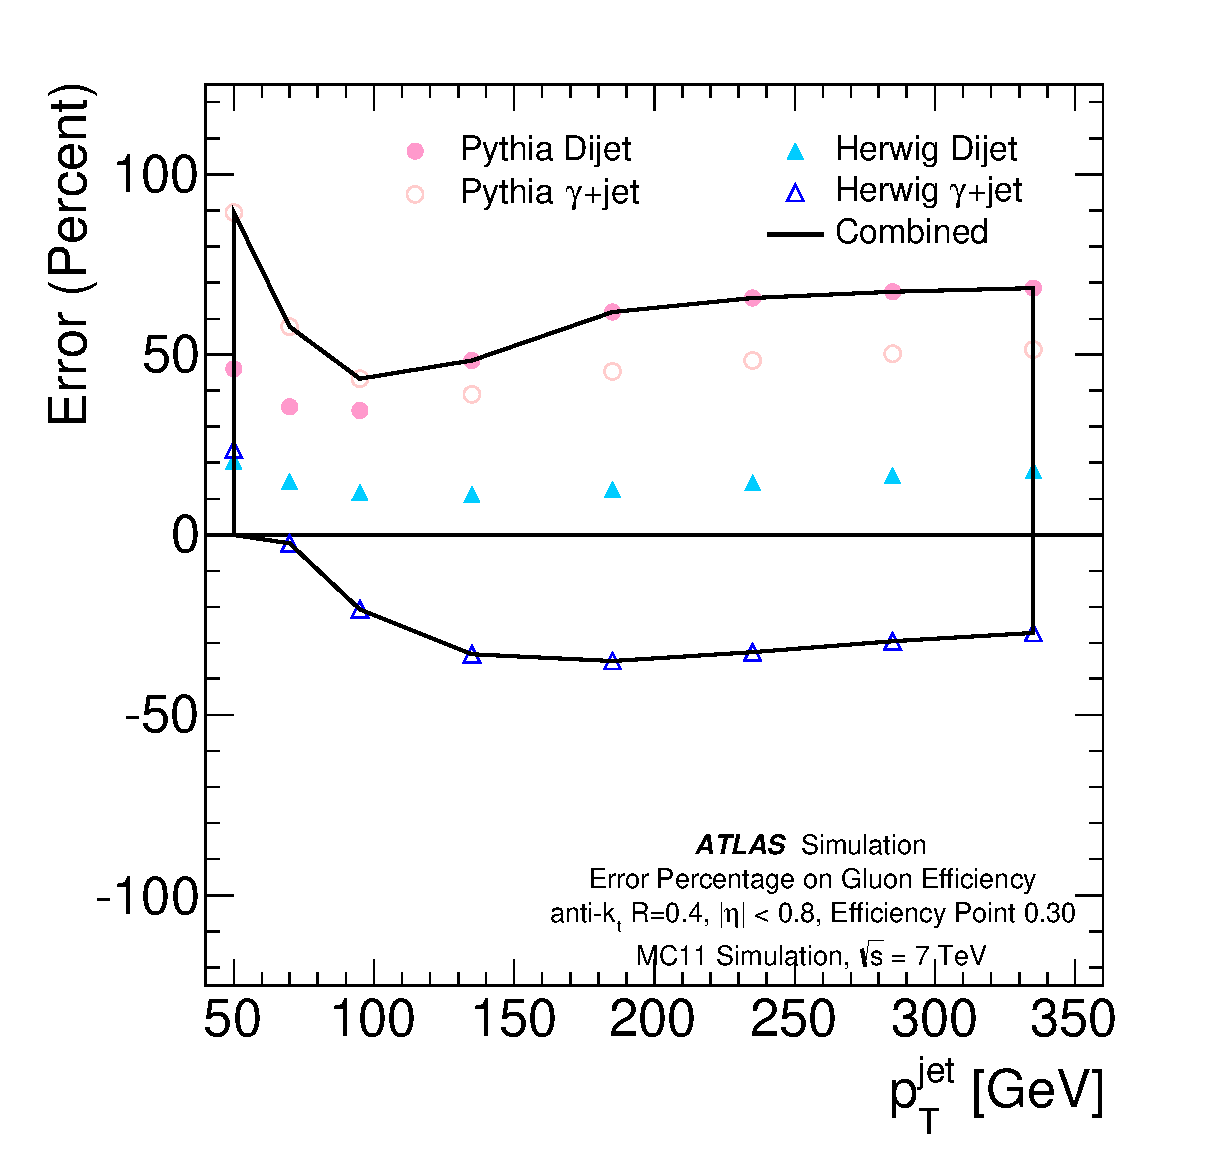
\includegraphics[width=0.48\textwidth]{qg/systs/smoothed_nonclosure_akt4TopoEM_eta0_30Eff} \\
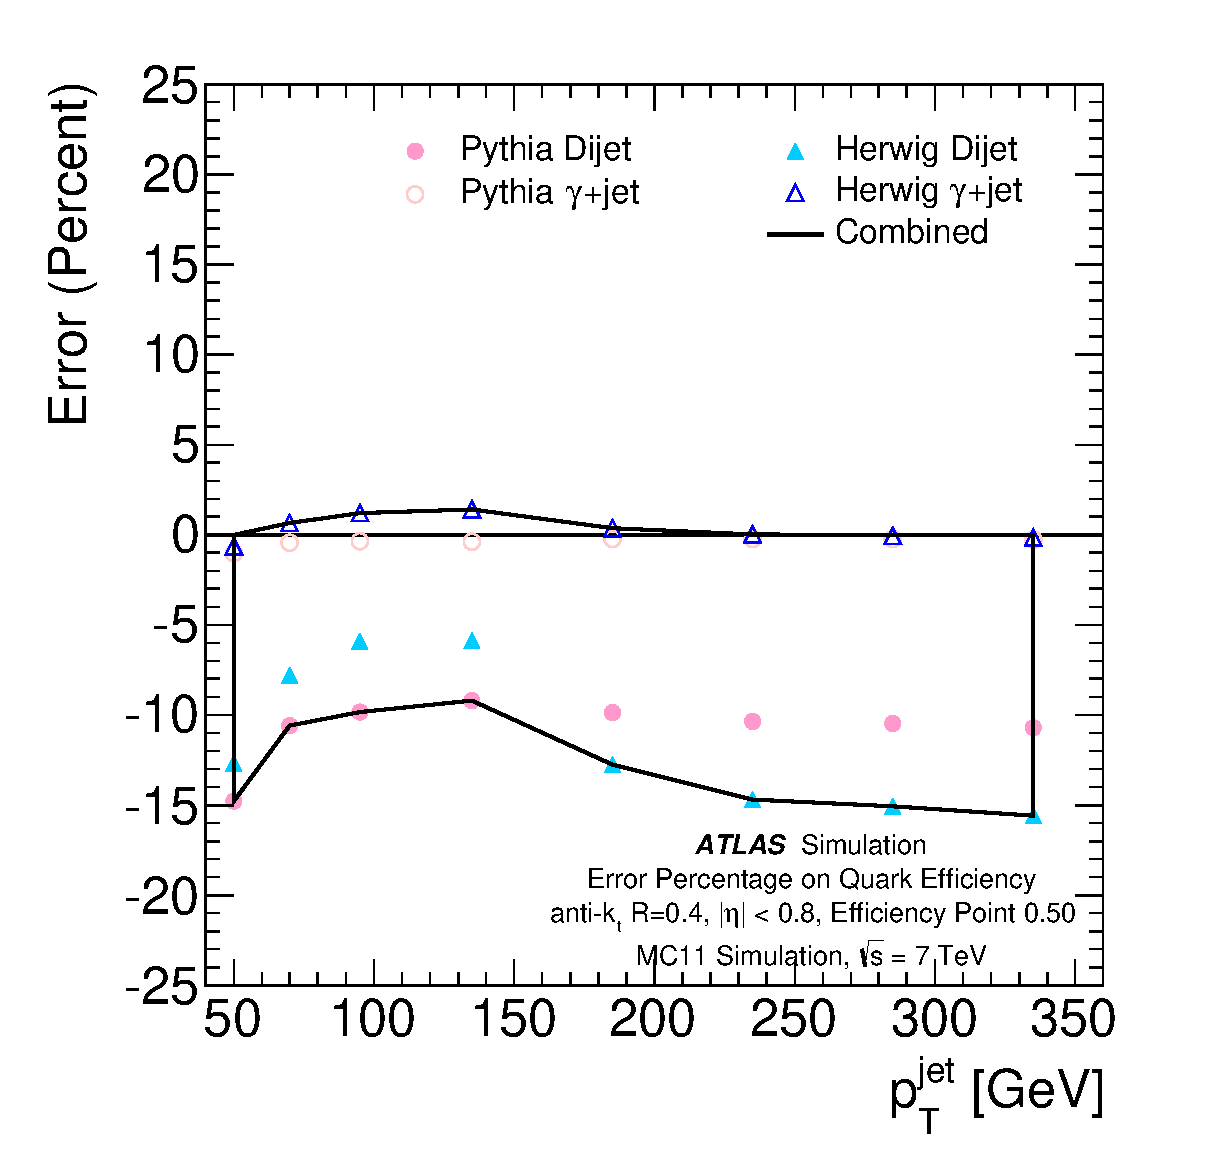
\includegraphics[width=0.48\textwidth]{qg/systs/smoothed_nonclosure_akt4TopoEM_eta0_50}
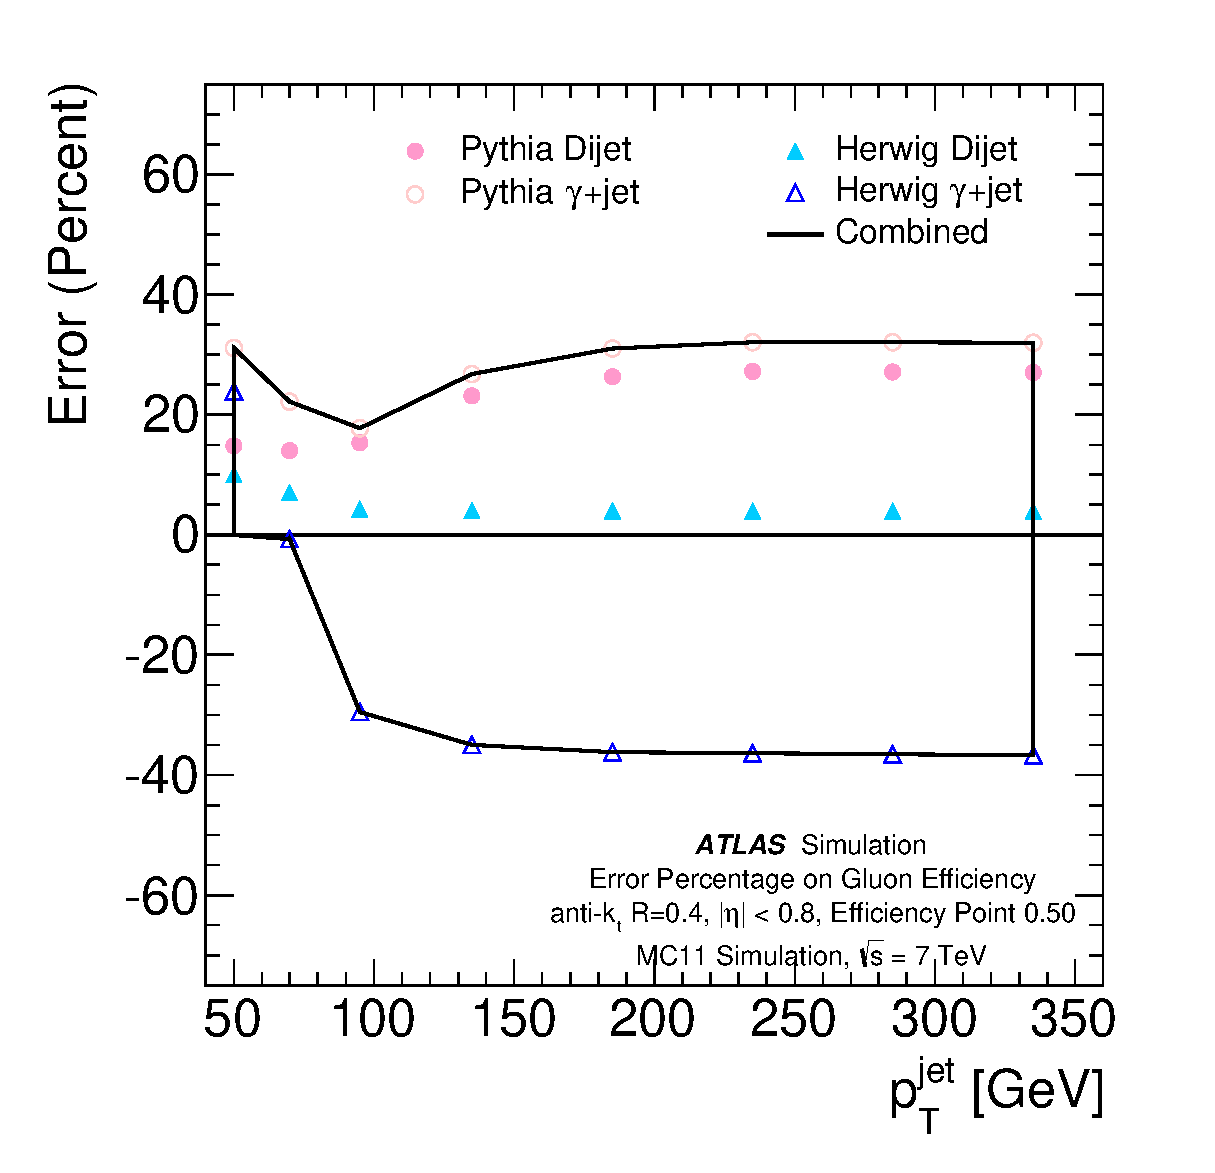
\includegraphics[width=0.48\textwidth]{qg/systs/smoothed_nonclosure_akt4TopoEM_eta0_50Eff} \\
\caption{ Sample-dependence effects on quark-jet (left) and gluon-jet (right) efficiency as a function
of jet $\pt$ for the 30\% (top) and 50\% (bottom) working points for jets with $|\eta|<0.8$.  Four different estimates
of sample-dependence effects are shown: the effects of applying the tagger in the
dijet and $\gamma$+jet \Pythia 6 MC samples, and in the dijet and $\gamma$+jet \Herwigpp MC samples.
Jets are reconstructed using the \AKT\ jet algorithm with radius parameter $R=0.4$.
A smoothing procedure has been applied to reduce the statistical uncertainties inherent in the
sample comparisons.
}
\label{fig:jet-reconstruction:qg:extractSyst}
\end{center}
\end{figure*}


\begin{figure*}[htbp]
\begin{center}
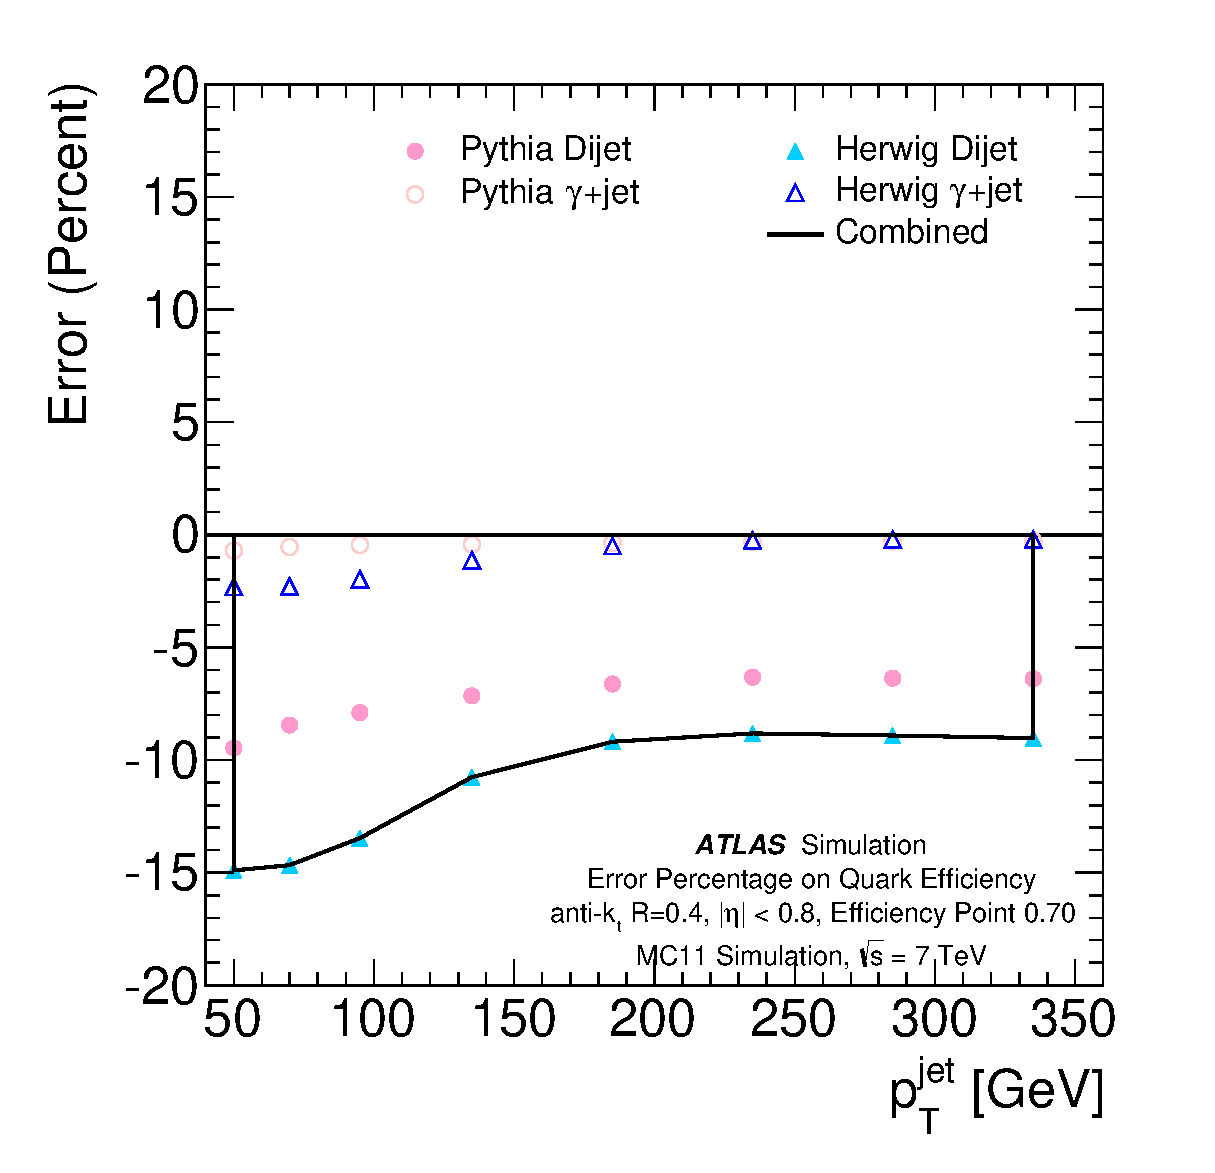
\includegraphics[width=0.48\textwidth]{qg/systs/smoothed_nonclosure_akt4TopoEM_eta0_70}
\includegraphics[width=0.48\textwidth]{qg/systs/smoothed_nonclosure_akt4TopoEM_eta0_70Eff} \\
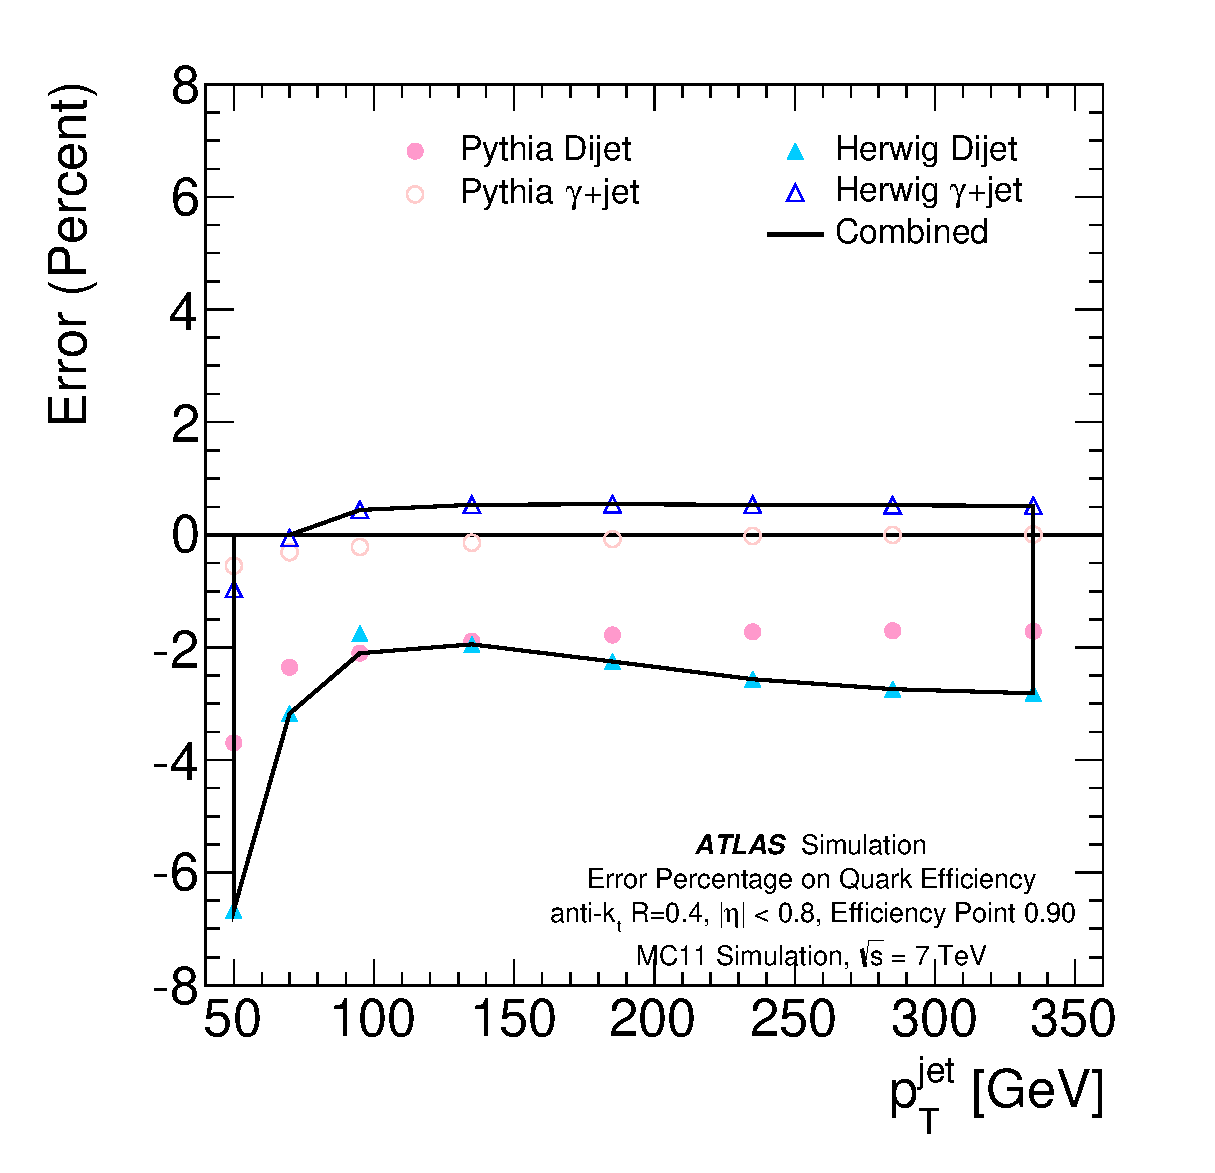
\includegraphics[width=0.48\textwidth]{qg/systs/smoothed_nonclosure_akt4TopoEM_eta0_90}
\includegraphics[width=0.48\textwidth]{qg/systs/smoothed_nonclosure_akt4TopoEM_eta0_90Eff} \\
\caption{ Sample-dependence effects on quark-jet (left) and gluon-jet (right) efficiency as a function
of jet $\pt$ for the 70\% (top) and 90\% (bottom) working points for jets with $|\eta|<0.8$.  Four different estimates
of sample-dependence effects are shown: the effects of applying the tagger in the 
dijet and $\gamma$+jet \Pythia 6 MC samples, and in the dijet and $\gamma$+jet \Herwigpp MC samples.  
Jets are reconstructed using the \AKT\ jet algorithm with radius parameter $R=0.4$. 
A smoothing procedure has been applied to reduce the statistical uncertainties inherent in the
sample comparisons. 
}
\label{fig:jet-reconstruction:qg:extractSyst2}
\end{center}
\end{figure*}

\subsection{Conclusions}

While the ATLAS quark-gluon tagger saw performance in data much worse than the prediction of the \Pythia MC, it was extremely elucidating to understand the data and MC disagreements in such detail. In the longer term, with an unfolded version of this analysis, generators could potentially be improved to show more reasonable showering distributions; in the short term, we know to be very skeptical of variables such as \ntrk which may not be very well modelled in MC.

\FloatBarrier

\section{Color Flow}

\subsection{Motivation}

What does it mean to see color at a collider?

The first question to ask, when considering color at the LHC, is what potential \textit{measurable} effects color can have, even if the color charge itself is not directly accessible. After all-- $SU(3)_C$ singlets ($W$, $Z$, $\ell$ particles), triplets ($q$ of all types), and octets ($g$) exist: surely there must be some observable differences between these states. Certainly, seeing red-blue-green is not particularly useful--- there's no consequential differences between a red quark and a green quark. But, seeing the difference between an octet and a singlet might indeed be useful: gluon octets, for example, can be backgrounds to signal singlets of various types. 

The first evidence of color at a particle collider was observed by the JADE experiment at PETRA-- in a process very familiar to the studies of Section~\ref{jet-reconstruction:qg:validation}. At PETRA, it was observed that the third leading jet (ordered in $p$) in tri-jet events had a \textit{broader} distribution of energy (comparing the distance of particles to the center of the jet axis) than that of the leading two jets: this was interepreted as evidence for the third jet being more likely to a gluon, whie the leading two were quarks~\cite{Bartel:1983ii}. This is exactly the same effect seen by ATLAS in Section~\ref{jet-reconstruction:qg:validation}, and is directly related to the magnitude of the color charge: the larger color charge for gluons implies that they fragment ``more,'' and consequentially have a higher multiplicity and less collimated shower. This first observation from PETRA sets the stage for color will be observed in other experiments: often it is not a direct effect on the 4-momentum of a jet, but is instead a property of the jet \textit{shape}. 

% A similar property, also first measured by PETRA but now explored by a variety of analyses at PEP, the Tevatron, and the LHC, is called \textit{color coherence}: this refers to the interaction of colored particles during the showering/fragmentation phase of an event, and implies that the angular distribution of jets should be somewhat different from the non-connected expectation. Many experiments have observed effects related to color coherence, at both $e^+/e^-$ and hadron-hadron colliders, in multi-jet events.~\cite{tasso,pep,PhysRevLett54270,PhysRevLett57945,PhysRevLett571398,PhysRevD.50.5562,Abbott:1997bk,Chatrchyan:2013fha}. In this type of analysis, color is sometimes measured with jet shapes, and sometimes indirectly via the push/pull of the jet axis away/towards some other jet.

% % look into these papers
% % bah compiling errors
% Colliders operating above the $W/Z$ mass scale can produce the vector bosons, and as these are color singlets, they provide an interesting testing ground for the measurement of color. These can be a testground for further color coherence studies, as studied by the Tevatron by measuring the calorimeter activity around leptonic $W$'s and jets~\cite{Abbott:1999cu}.  L3 and DELPHI, in turn, studied the energy between $W$ bosons in $WW$ events, comparing pairs of jets from the same or different $W$, and observed that different color flow models predicted different behavior, in a process referred to as \textit{color reconnection}~\cite{Achard:2003pe,Abdallah:2006uq}. In these studies, $W$ bosons were used as test samples to study color, usually by looking outside of the jet for additional radiation: color was visible not as a property of the jet, but of the environment surrounding it.

Most historical measurements have been sensitive to the presence of color--- indeed, the seminal JADE measurement is even principle to the magnitude of the color charge--- but most of them are used to constrain color \textit{models}, and not determine the actual color properties of objects. That is to say, these measurements all help tune MC generators and shower models to more accurately reproduce the effects of hadronization and the residual effects of color, but none of them have measured the actual color representation of the $W$, for example. While it is clear from leptonic helicity measurements and $W$+jets production cross-sections that the $W$-boson is a color singlet, the hadronic decays of a $W$ have not been used to \textit{directly} measure the color type: the most direct way of \textit{seeing color} at colliders has not been performed.

Figure~\ref{fig:detector:schematic} gives an example of the color flow in the SM on the left hand side: this blue line connecting the $W$-daughter quarks is the color connection between the two jets, and is determined by the color type of the $W$. Because it is a singlet, it cannot carry a color line itself, and so colored objects decaying from it must be connected (via blue/anti-blue, for example). On the right side is an example of a hypothetical alternative model, where the $W$ acts as a color octet: then, it is able to carry \textit{two} colors, and the $W$-daughter quarks do not share a color connection. The effect for this connecting color line is often referred to as \textit{color flow}. Does the blue color line in this figure exist in data? How can we tell? 

%%%%%%%%%%%%%%%%

\begin{figure}
\centering
\includegraphics[width=0.7\textwidth]{paper/schematic.pdf}
\label{fig:color:motivation:schematic}
\caption{An example of the color flow in SM $t\bar{t}$ events on the left, and a hypothetical exotic model where the $W$ is an octet on the right.}
\end{figure}

%%%%%%%%%%%%%%%%  

This question is not just academic: telling the difference between a singlet and an octet can already be useful in LHC searches. For example, the Higgs boson has not yet been observed in its decay to $b$-quarks: as a singlet, it should have a different color flow from that of the main gluon backgrounds. Likewise, if a new particle is discovered in a dijet resonance, it will be immediately important to characterize its color representation: measuring the color flow, in a similar way to the schematic of Figure~\ref{fig:detector:schematic}, will be critical. 

The following section briefly outlines a recent ATLAS measurement of color flow in semi-leptonic $t\bar{t}$ events using the \textit{jet pull angle}~\cite{Aad:2015lxa,Nachman:1728288}. This analysis was performed by a collaboration between the SLAC, Manchester, and Harvard groups, in association with the theorist who devised the variable, Matt Schwartz~\cite{Gallicchio:2010sw}.\footnote{I would like to particularly acknowledge the contributions of Benjamin Nachman (who developed many of the object corrections, object selections, uncertainties, optimizations, figures, alternative color model, and more), and Thomas Neep (who developed much of the unfolding and final presentation and interpretation of results). My main contributions were in the event selection and related uncertainties, as well as initial studies of the pull angle and corrections. A much more detailed accounting of this work will appear in Nachman's upcoming thesis.}



\subsection{The Pull Angle}

What we have learned so far from previous color measurements is that two basic categories of information are useful in seeing color related effects:
%
\begin{enumerate}
\item Energy distributions inside, or surrounding, jets
\item Orientation of jet axes, and angular kinematics 
\end{enumerate}
%
One recently developed variable, the \textit{jet pull}, combines both of these types of information~\cite{Gallicchio:2010sw}. The variable composes a vector of a \pt and radial distance weighted sum over constituents of a jet and determines the oriention of this vector in relation to other jets, thereby combining the structural information about the jet with the broader context of the event (in a strategy sometimes referred to as jet superstructure). The D0 and CMS collaborations, as well as theorists, have used this variable as a part of multivariate analyses to improve sensitivity to Higgs decays to b-quarks already.~\cite{D0higgs,CMShiggspap,CMShiggspap2}. D0 also attempted a measurement of the color flow using the pull in top quark decays, comparing reconstructed data events to templates of the pull composed using singlet and octet $W$-boson models; the result, however, was strongly statistically limited and not able to distinguish between singlets and octets.

The first step in measuring color flow with pull is to construct the \textit{pull vector} for a jet, defined as:
%
\begin{align}
\label{eqn:pull}
\vec{v} = \sum_{i\in J} \frac{p_T^i |r_i|}{p_T^{J}}\vec{r}_i,
\end{align}
%
where $i$ iterates over elements (topo-clusters or tracks or truth particles) associated to some jet $J$, $\vec{r}_i = (\Delta y_i,\Delta\phi_i)$ (i.e. the vector composed of the difference in rapidity and azimuthal angle between the element and the jet axis). The pull vector encodes the substructure information related to the color flow of the jet: the vector points in the direction that the jet is \textit{leaning} in some sense. By itself, this information is not particularly interesting; what makes it useful is its relation to other jets. Given a pull vector composed for a jet $J_1$, the \textit{jet pull angle} $\theta_P(J_1, J_2)$is the opening angle between $\vec{v}_1$ and a jet $J_2$ in $(\Delta y,\Delta\phi)$ space~\cite{Gallicchio:2010sw}. There are two ways for a constituent to contribute strongly to the pull vector: either it has large $\pt$ or a large $r_i$, or both. In a color connected pair of jets--- that is, a pair of jets with a color line connecting them as in the left of Figure~\ref{fig:detector:schematic}--- it is expected that the jets should lean \textit{towards each other}: their energy should be oriented between them, and the pull angle should tend to 0. On the other hand, un-connected jets--- such as the right side of Figure~\ref{fig:detector:schematic}--- should have no preferred orientation, and so the pull angle is expected to be essentially isotropically distributed. Note that while in principle $\theta_P$ ranges from $-\pi$ to $\pi$, the distribution should  be symmetric, and so in all of the following analysis we define $\theta_P$ as the absolute value of the pull angle.



% The following chapter discusses a new ATLAS measurement (as yet unpublished) which not only measures the color flow using the jet pull, but also unfolds the data to particle level. Our goal is to demonstrate that we can ``see'' the blue color line of Figure~\ref{fig:detector:schematic}, but also to measure the energy distributions inside of jets in a context where these distributions are sensitive to color effects, in order to improve the modeling of such effects in MC simulation. Moreover, while 4-vector based measurements of color connection effects in multi-jet events have been performed at the LHC~\cite{Chatrchyan:2013fha}, there have been no measurements yet of the actual jet energy distributions which the pull angle tells us about. By demonstrating that we can tell the difference between singlets and octets, we can motivate the use of jet pull to search for the Higgs or characterize new particles; by measuring the distribution of the jet pull angle we can present to theorists the first measurement unfolded energy flow measurement at a hadron collider at $\sqrt{s} = 8$~TeV.


\subsection{Reconstructing Color}

Following the example of the D0 analysis~\cite{Abazov:2011vh}, the measurement we perform uses $t\bar{t}$ events as Figure~\ref{fig:detector:schematic} suggests. We employ a semi-leptonic selection, where one of the $W$'s in the event decays leptonically, to select a very pure sample of top quarks: with this topology, we are able to obtain a $>90\%$ pure top sample. The leptonic $W$ acts essentially as a tag for the event, and we can then study the properties of the hadronically decaying $W$.

To compare the singlet $W$--- generated using normal \PowPythia $t\bar{t}$ samples--- to an octet $W$, we need to generate a simulation of the octet. While it is possible to compose a full BSM model which includes octet $W$'s and generate MC in this way, this is slightly non-optimal: observables just as the jet \pt and angles will potentially change due to the different particle content, while we wish to assess \textit{only} the power of color flow via the substructure. The most straightforward way to do this is to take the \textit{same events} used to generate the nominal singlets and to create new events with an inverted color structure. These events have their color structure flipped at the Matrix Element level, before showering and hadronization. Once the flip is performed, showering and hadronization are run as normal-- except now reflecting the different color structure. The advantage of this scheme is that the \pt and angular distributions of jets should be largely the same as the nominal sample, except for the color flow effects: this is as fair a comparison as we can make. Samples are produced with both \PowPythia and \PowHerwig generator+showering model schemes. 


The inputs to Equation~\ref{eqn:pull} are a free choice: while it is natural to use calorimeter clusters, it is also possible to use tracks from the inner detector. Both are sensitive techniques, even though the charged-only measurement is throwing away 1/3 of the particles (the neutrals). The advantage of performing two measurements is that the experimental systematics are completely different for each: uncertainties on the tracker have a very different character from that of the uncertainties on calorimeter objects. Moreover, while the charged particle measurement throws away a significant amount of information, each particle is measured with a significantly better resolution: the \pt measurement of a track does not suffer the response fluctuations which dominate the resolution of a calorimeter. Thus, we proceed with both analyses in parallel--- many aspects of them will be shared, but some will be different, and the ultimate power of each result can be compared at the end.


The goal of our analysis to obtain a pure sample of hadronically decaying $W$-bosons, and to measure the pull angle between the jets initiated by the decay of the $W$. To better allow the measurement to be utilized by theorists for generator tuning, and to compare to other models of color flow more easily, the analysis is corrected for detector resolution and efficiency effects and \textit{unfolded} to particle level. At this stage, a comparison can be made between the data, the singlet MC, and the octet MC, and we can determine whether the data is able to tell the difference between the two possibilities. All stages of the analysis are performed with both topological calorimeter clusters, which measure all interacting particles in a jet, and tracks reconstructed from the inner detector, which measure only the charged particles but with much improved resolution.

\subsection{Finding Top Quarks}

The following section discusses the object selections and cuts used to define the $t\bar{t}$ sample used in the analysis.

\subsubsection{Trigger}

As the analysis is semi-leptonic in order to guarantee a high purity of $t\bar{t}$ events, it is sensible to also use the lepton triggers. A logical OR between {\tt EF\_mu24i\_tight}, {\tt EF\_mu36\_tight}, {\tt EF\_e24vhi\_medium} and {\tt EF\_e60\_medium} is used for the whole data taking period. The first and second triggers are the muon triggers; the third and fourth are the electron triggers. The numbers in the trigger name refer to the \pt threshold of the online trigger. The first and third triggers require isolation at the trigger level, thereby allowing a lower \pt threshold; the second and fourth have no isolation requirement, but a much higher \pt treshhold. The \pt $>$ 25~GeV cut on the offline lepton-- described below-- guarantees that the combination of isolated and non-isolated triggers are fully efficient.

\subsubsection{Object Selections}

This analysis makes use of many different object types: jets, $b$-tags, electrons, muons, and \met. The exact quality and selection requirements for each are discussed below.

\textbf{Electrons} are tracks matched to isolated EM calorimeter clusters\footnote{EM clusters for electrons are composed of 3x3 cells.}, refit via a Gaussian Sum Filter technique to take into account the larger material interactions and radiations of electrons compared to the initial pion hypothesis~\cite{Aad:2014nim,Aad:2014fxa,ATLAS-CONF-2014-032,ATLAS-CONF-2012-047}. For this analysis, they are required to pass the \texttt{Tight++} requirement with ``author'' equal to 1 or 3--- this is a set of cuts on the shape of the electron cluster which suppresses backgrounds from jets and photons, and on track quality. The \pt of the electron is set to $E_\mathrm{cluster} / \cosh \eta_\mathrm{cluster}$, and $|\eta| < 2.47$ is required. In addition, the so-called ``crack'' region of $1.37 < |\eta| < 1.52$ is vetoed as electron identification is more difficult in this region. To ensure consistency with the primary vertex, a requirement on the track of $|z_0| < 2$~mm with respect to the primary vertex is imposed. Furthermore, basic quality criteria are applied to reject electrons reconstructed from noisy or dead calorimeter clusters. The energy in a $\Delta R < 0.2$ cone (measured with calorimeter cells) and the \pt within a $\Delta R < 0.3$ cone (measured with tracks) are required to be small. This isolation requirement--- used to suppress electrons from leptonic $B$ decays and fakes from jets in general--- is tuned to select $90\%$ of all electrons. Finally, electrons are required to be isolated from the signal jets (defined below): the jet is removed in favor of the electron if $\Delta R < 0.2$ between any pair, and electrons are removed if $0.2 < \Delta R < 0.4$. This selection is optimized to efficiently keep electrons which are ``faking'' jets (very easy to do, as calorimeter clusters from the electron enter into jet clustering), while removing events where a real jet has emitted an electron (in leptonic $B$-decays, for example). Since this analysis is single-lepton, the electron is also required to match to the trigger electron.

\textbf{Muons} are generally inner detector tracks matched to muon-spectrometer tracks (though various combinations are possible--- inner detector only, muon-spectrometer only, inner detector with a calorimeter tag, etc.). The muons in this analysis are required to be \texttt{Tight} combined muons, indicating that tracks are indepenently constructed in both systems and well matched via the \texttt{Muid} algorithm. Cuts of $\pt > 25$~GeV and $|\eta|<2.5$ are applied. Several requirements on the track quality are applied: a b-layer hit is required if expected, and the number of silicon hits is required to be greater than 4, with the number of holes (crossings with no hit, but one expected) to be $< 3$. The $|z_0|$ is again required to be $< 2$ mm from the primary vertex. Additional requirements on the TRT hits are also applied. The isolation is defined using a variable cone scaling, summing the $\pt$ of all tracks within a cone of size $\Delta R < 10~\mathrm{GeV} / \pt^{\mu}$: the scaling allows the better reconstructed high-\pt muons to not be removed by overlaps with jets as the boost of the top quark increases. The cut applied is $I_\mathrm{mini} / \pt^{\mu} < 0.05 $.  Muons are also required to be isolated from jets with a cone of $\Delta R < 0.4$. Similarly to the electrons, a good muon candidate must also match to a trigger muon.

\textbf{Jets} are reconstructed as per the discussion in Chapter~\ref{chapter:jet-reconstruction}. Cuts of $\pt > 25$~GeV and $|\eta| < 2.1$ are imposed; the $\eta$ requirement is tighter than for other objects to insure that the jet is fully enclosed in the tracker so that the jets can be effectively $b$-tagged and its tracking properties measured for the track pull angle measurement. For jets with $\pt < 50$~GeV a JVF cut of $\mathrm{JVF} > 0.5$ is required to reduce the impact of pileup jets. The origin correction of the jet is a particularly important element of the analysis, as the pull vector is very sensitive to the choice of axes. As described below, the topo-clusters are origin-corrected, removing smearing due to the changing $z$-location of the primary vertex, and the sum of their 4-vectors are used as the jet axis. The calibrated $\eta$ is not used in the pull calculation, as it is offset from the center of the clusters, and this can produce lare biases in the pull angle.

\textbf{B-tags} are defined using the MV1 algorithm at a $70\%$ efficiency operating point.

\textbf{Missing energy} is calculated using all the calibrated signal objects in the analysis, and the un-associated topo-clusters in the calorimeter which form the ``soft term'' which measures the underlying event. The entire method is referred to as \texttt{METRefFinal}~\cite{Aad:2012re,ATLAS-CONF-2013-082,ATLAS-CONF-2014-019}.


\subsubsection{Selection Cuts}

The following cuts are used to define the data sample:
%
\begin{enumerate}
\item Require that there were no large scale detector or calorimeter issues during the event (GRL and detector quality cuts)
\item Require one primary vertex associated with five or more tracks with $\pt > 0.4$~GeV
\item Require either the electron or muon trigger to have fired
\item Require exactly 1 good muon or electron (depending on which trigger fired)
\item Require that no jets with $\pt > 20$ GeV fail quality criteria
\item Require that there exist 4 or more jets with $\pt > 20$~GeV and $|\eta| < 2.5$
\item Require $\met > 20$~GeV
\item Require $\met + m_T > 60$~GeV\footnote{The $m_T$ variable is the transverse mass, associated with the visible mass of the leptonically decaying $W$ boson. It is defined as $m_T^2 = 2 \pt^{\mathrm{lep}} \met (1 - \cos(\Delta \phi))$.}
\item Require 2 $b$-tagged jets
\item Require 2 non-$b$-tagged jets
\end{enumerate}
%
This is mostly a very standard selection for semileptonic $t\bar{t}$, and has been used by ATLAS in many analyses very consistently and effectively \editnote{Cite this.}. One change with respect to the standard selection is a change to point 9: the nominal selection chooses only 1 $b$-tag, but we select 2 in order to more accurately classify and label the event. For this same reason, we require 2 non-$b$-tagged jets: this allows for less ambiguity, as we have much stronger confidence that the $b$-jets from the top quark decay are appropriately identified. We label these two jets, in \pt ordering, as $B_1$ and $B_2$.


The remaining question is how to assign the label of $J_1$ and $J_2$, the candidate jets from the $W$ decay, in the case when there are more than 2 non-$b$-tagged jets. It is simplest, and most consistent with the \textit{pseudo-top} definition from the {\sc TopLHCWG}, to use the leading two non-$b$-tagged jets~\cite{pseudotop,Aad:2015eia}.

% Note that the following analysis uses the pull angle of the $J_1$ with respect to $J_2$: while it is possible to use the pull angle of $J_2$ with respect to $J_1$, the resolution actually suffers (as described in Section~\ref{chapter:color:reconstruction:resolution}) and the added statistics would not strongly benefit the analysis.

Finally, a dedicated truth selection mimicing the reco-level selection is implemented for truth-level studies. This selection provides a fiducial region for targetting the unfolding. Final state electrons and muons are used as the leptons; photons with $\Delta R < 0.1$ are assumed to originate from radiation from the lepton and are added back to the 4-vector. Final state neutrinos that do not originate from a hadron are used to determine the missing energy. Jets are clustered from final state particles that are not leptons or neutrinos. $b$-jets are labelled via a ghost-association scheme: truth $B$-hadrons with $\pt > 5$~GeV are allowed to participate in the clustering of the truth jets (though with a scaled, ghost-level \pt) and the jet to which they are clustered is labelled as originating from a $B$-hadron. All the same kinematic cuts from the reco-selection are then applied to the truth-objects.

\subsubsection{MC Backgrounds}

While the selection above is optimized to select $t\bar{t}$ events with very high purity, there are inevitably many different sources of background which must be assessed. The backgrounds are assessed in three ways: directly with MC simulation, using data-driven techniques, or a combination of the two. First, we discuss the MC-driven background estimates.

\textbf{Single top} is assessed in the $s$, $t$, and $Wt$ channel using samples generated with \PowPythia. The $Wt$ channel assess its interference with the nominal $t\bar{t}$ sample using the ``Diagram Removal'' scheme, while the contrasting ``Diagram Subtraction'' scheme is used to assess the theoretical systematics on the sample. The $Wt$ channel contributes the most, and is a non-negligible background.

\textbf{Diboson} production is simulated using \Sherpa version 1.4.1; this generator is found to model the production of dibosons in association with heavy flavor quarks-- i.e., that final state with the largest contribution to our selection-- better than \Herwigpp and other generators. This background is negligible.

\textbf{$\mathbf{Z}$+jets} are assessed with \Alpgen interfaced with \Pythia, generated with separate samples for each additional emission up to 5 partons. All the samples require the $Z$ to decay leptonically in order to provide the leptons required for the analysis selection (hadronically decaying $Z$+jet events do not contribute to the selection). Dedicated filtered heavy flavor samples are produced, and the overlap with the inclusive samples is assessed with the ``Heavy Flavor Overlap Removal'' (HFOR) scheme. The $Z$+jets background is very small.

\textbf{$\mathbf{W}$+jets} are assessed similarly to the $Z$+jets: \Alpgen is interfaced with \Pythia, and separate samples are generated for each real emission, up to 5 partons. All the $W$'s are required to decay leptonically, mimicing the leptonic $W$ in the $t\bar{t}$ decay. Separate samples are generated also for heavy flavor, with both $c$ and $b$ quarks; once again, the overlap is assessed using HFOR. The $W$+jets background is the largest in the analysis, and so a data-driven normalization (described below) is derived to ensure that it is accurately modeled. 


\subsubsection{Data-Driven Backgrounds}

The normalization on \textbf{$\mathbf{W}$+jets} is assessed with a \textit{lepton-charge-asymmetry} technique~\cite{wjetscharge}. More $W^+$ than $W^-$ events are produced at the LHC because the input hadrons are both positive. The ratio of these two, $r_{MC}$, is better predicted than the absolute cross-section. To derive a scale factor, we note that the sum of both charge types over the difference of charge types should be equal, up to the scale factor $\alpha$:
%
\begin{equation}
\alpha \frac{N_\mathrm{data}^+ + N_\mathrm{data}^-}{N_\mathrm{data}^+ - N_\mathrm{data}^-} = \frac{N_\mathrm{MC}^+ + N_\mathrm{MC}^-}{N_\mathrm{MC}^+ - N_\mathrm{MC}^-}
\end{equation}
% 
which we can rewrite with the ratio $r_{MC}$ as:
%
\begin{equation}
\alpha \frac{N_\mathrm{data}^+ + N_\mathrm{data}^-}{N_\mathrm{data}^+ - N_\mathrm{data}^-} = \frac{1 + r_{MC}}{1 - r_{MC}}
\end{equation}
%
which allows us to solve for the scale factor:
%
\begin{equation}
\alpha W = \frac{1 + r_{MC}}{1 - r_{MC}} \left( N_\mathrm{data}^+ - N_\mathrm{data}^- \right)
\end{equation}
%
where $W$ is the inclusive $W$+jets sample (i.e. the sum of both charges). This scale-factor is derived in bins of jet multiplicity, and separetely for events with and without a $b$-tag\footnote{The scale-factor from the one-tag sample was determind to be consistent with the two-tag sample, which more closely corresponds to our selection.}. The data-sample used is enriched in $W$+jets events to a very high purity, though background contributions from $t\bar{t}$, etc. mostly do not matter because they are largely charge-symmetric and drop out of the scale factor.

The shape of the $W$+jets background therefore is taken from MC, but the normalization is corrected using this data-driven approach, substantially reducing the theoretical uncertainties on the largest background to the analysis. The values derived are $1.3 \pm 0.03$ for the $bb/cc$ component, $0.74 \pm 0.04$ for the single $c$ component, and $0.96 \pm 0.02$ for the light component.

\textbf{Multi-jet backgrounds} are very poorly modelled in the simulation, as fake leptons are difficult to predict correctly. A data-driven approach called the \textit{matrix method} is therefore adopted to assess this background~\cite{MatrixMethod}. The goal of the method is to assess $N_\mathrm{fake}^\mathrm{tight}$: the number of fake ``tight'' leptons produced by multi-jet events.  This number is derived using two samples, differing only in the definition of the leptons: either the ``tight'' nominal selection (described above), or a ``loose'' selection with some of these requirements removed (the differences in the loose selection for muons and electrons, which are assessed separetely in this technique, will be described below). A tight lepton, by definition, passes the loose requirements. The tight sample mostly contains real leptons, while the loose sample is enriched in the fakes we are trying to measure, but both samples are a mixture. Thus, we can write:
%
\begin{align}
N^\mathrm{loose} &= N_\mathrm{real}^\mathrm{loose} + N_\mathrm{fake}^\mathrm{loose}\\
N^\mathrm{tight} &= N_\mathrm{real}^\mathrm{tight} + N_\mathrm{fake}^\mathrm{tight}
\end{align}
%
In addition, we can define the \textit{efficiency} of the tight selection as:
%
\begin{equation}
\epsilon_\mathrm{x} = \frac{N^\mathrm{tight}_\mathrm{x}}{N^\mathrm{loose}_\mathrm{x}}
\end{equation}
%
where $x$ is either real or fake. Here we are simply stating that the tight selection has a different efficiency of selecting real and fake leptons (i.e. it should be rather efficient for real leptons, but very low efficiency for fake leptons). The efficiencies $\epsilon_\mathrm{x}$ are measured separately in data (via a method described below), so we can take these as given for now. Plugging all these equations together, it is possible to solve for our desired quantity:
%
\begin{equation}
N_\mathrm{fake}^\mathrm{tight} = \frac{\epsilon_f}{\epsilon_r - \epsilon_f} \left(\epsilon_r N^\mathrm{loose} - N^\mathrm{tight} \right)
\end{equation}

In order to derive kinematic distributions-- and not just an overall number-- this quantity can be converted to a series of weights for each event $i$:
%
\begin{equation}
w^i = \frac{\epsilon_f}{\epsilon_r - \epsilon_f} (\epsilon_r - \delta_i)
\end{equation}
%
where $\delta_i = 1$ if the event passes the tight selection, or $\delta_i = 0$ otherwise. These weights are further normalized such that $\sum_i w_i = N_\mathrm{fake}^\mathrm{tight}$. When run over the entire dataset, these weights thus provide the expected multi-jet contribution to the selection.

Loose electrons are defined using the \texttt{medium++} quality criteria, with an additional requirement of a photon conversion veto (which is normally part  of the \texttt{tight++} requirements)~\cite{Aad:2014fxa,ATLAS-CONF-2014-032}. There is also no isolation applied. Together, these cuts substantially enrich the loose sample with fake leptons. Loose muons are similar: only the isolation requirement is dropped.  

Efficiencies for real leptons are measured using a tag-and-probe method in leptonic $Z$ decays: a tight lepton (the tag) is used to study loose leptons (the probe). The number of probes (i.e. loose leptons) which pass a tight requirement gives a measurement for $\epsilon_\mathrm{real}$. 

Efficiencies for fake leptons are measured using a control region which inverts the \met and $m_T$ requirements, lowers the requirements on the number of jets, and loosens the $d_0$ cut on leptons. This enriches a sample of fake leptons with kinematics similar of the signal region, but still contains a great deal of real leptons: these must be subtracted out by using MC simulation.

\subsubsection{Data/SM Yields}

Now that all the backgrounds have been assessed, we can compare the data and SM prediction yields after the selection described above. Table~\ref{tab:color:yields:yields} shows the predicted and observed values; the sample has an excellent $t\bar{t}$ purity of $91\%$. The muon channel comprises $53\%$ of the data, so slightly more than the electron channel. Note that the $t\bar{t}$ in this section is always the nominal color flow \PowPythia sample.


\begin{table}
  \centering
  \vspace{3mm}
  \begin{tabular}
  {
 c
 S[table-format=1,
   table-figures-uncertainty=0,group-digits = false,tight-spacing]
}
    \toprule
    Process                      & Counts                                   \\
    \midrule
    $t\bar{t}$                   & 95400 \hspace{1mm}$\pm$\hspace{1mm} 200  \\
    $Wt$-chan single top         & 2730\hspace{1mm} $\pm$\hspace{1mm} 40    \\
    $s$- and $t$-chan single top & 150\hspace{1mm} $\pm$\hspace{1mm} 1      \\
    $W$+jets                     & 3710\hspace{1mm} $\pm$ \hspace{1mm}70    \\
    $Z$+jets                     & 560 \hspace{1mm}$\pm$ \hspace{1mm}10     \\
    Dibosons                     & 190\hspace{1mm} $\pm$\hspace{1mm} 10     \\
    Multijets                    & 2500\hspace{1mm} $\pm$ \hspace{1mm}40    \\
    \midrule
    Total SM                     & 105000 \hspace{1mm}$\pm$ \hspace{1mm}220 \\
    Data                         & 102987                                   \\
    \bottomrule
  \end{tabular}
  \caption{Estimated sample composition.  $W$+jets and multijets estimations are data-driven. Only uncertainties due to finite statistics are listed.}
  \label{tab:color:yields:yields}
\end{table}

We can also make comparisons between the data and SM expectation for the various kinematic quantities of the events (and in particular, the $W$-candidates) to validate that the modeling is well predicting the data distributions well. Figure~\ref{fig:color:yields:pts} shows the leading $W$-jet candidates' \pt distributions for the muon (left) and electron (channels) in right. The purity of the $t\bar{t}$ sample is immediately clear, but more concerning is the slope seen in the data/SM ratio. This is a well known effect related to the mismodelling of the top quark \pt in many MC simulations. Tests were performed to reweight the \pt distributions in simulation to agree with the data and to check if this had any impact on the pull angle observables: the result was a negligible change, and so this effect is not considered important\footnote{While the pull vector is normalized by the jet \pt, the angle is not directly affected and so the observables are not directly impacted by this mismodelling.}. Note also that the uncertainties in this plot (and all subsequent plots) include all detector effects described in Section~\ref{chapter:color:uncertainties:other}, but no theoretical uncertainties from Section~\ref{chapter:color:uncertainties:theory}. In all cases, the MC simulation is normalized to the luminosity.


\begin{figure}[h!]
\begin{center}
\includegraphics[width=0.45\textwidth]{cf_int/DataMC/J1pT}\includegraphics[width=0.45\textwidth]{cf_int/DataMC/J1pTe}
 \caption{The leading $W$ daughter jet $p_T$ for the muon channel (left) and the electron channel (right). The slope in data/MC is a well known deficiency of the current tune of the \PowPythia sample, but has no effect on the observable of interest. }
 \label{fig:color:yields:pts}
  \end{center}
\end{figure}



	\subsection{Substructure Objects}

Having obtained a high-purity sample of hadronically decaying $W$'s in both data and simulation, we can now begin to study the actual pull angle distribution. The first step is to define the input objects for the pull vector calculation.

	\subsubsection{Topological Calorimeter Clusters}

Topological calorimeter clusters are familiar objects by now: these are the inputs to jet clustering, and are used to calculate substructure moments in many different analyses. Much has already been said on the topic in Section~\ref{jet-reconstruction:jet-inputs:topoclustering}, and everything discussed there is used for the color flow measurement. In particular, the locally calibrated clusters are used: as is common for substructure, having all calorimeter elements as close as possible to the true particle scale helps ensure that all particles contribute to the reconstructed substucture moment. 

Additionally, a new correction for the primary vertex origin is applied in this analysis. As discussed in Section~\ref{jet-reconstruction:origin}, the $z$-coordinate of the primary vertex is not necessarily at the origin of the detecotr, and a correction to jets based on the measured location of the vertex can substantially improve the $\eta$ resolution of the jet. As we use standard \akt $R=0.4$ jets in this analysis, this means that the jet axis is origin corrected, but the clusters by default are not. One can also correct the \textit{clusters themselves} for the changing location of the primary vertex. The correction is given by: 
%
\begin{align}
z &= R\sinh\eta\nonumber\\
z &\mapsto z' = z - z_\text{corr}\nonumber\\
\eta &\mapsto \eta' = \text{asinh} (z'/R) = \text{asinh}(z/R - z_\text{corr}/R) = \text{asinh}(\sinh(\eta) - z_\text{corr}/R)
\end{align}
%
where $R$ is the radial depth of the cluster. The $p_T$ of the corrected cluster is defined similarly:
%
\begin{align}
p_T=E/\cosh(\eta)\mapsto E/\cosh(\eta')=p_T\cosh(\eta)/\cosh(\eta')
\end{align}
%
As this correction is data-driven (it is not calibrated in MC), it corrects the resolution of both data and MC to the same level.

\subsubsection{Tracks}

Tracks are automatically origin-corrected: there is no assumption of the location of the vertex at the origin of the detector, as the appropriate primary vertex is determined via the measured $z_0$ of the track. However, the axis bias may still exist: since the jet axis is formed from clusters, and not tracks, there is no guarantee that it lies in the center of the tracks. To correct for this, all track pull measurements are constructed with respect to axes formed by summing the 4-momenta of the associated tracks.

Track quality requirements are rather standard. They are required to have $\pt \geq 500$~MeV, $|\eta| < 2.5$, and $\chi^2/\mathrm{ndf} < 3$. Furthermore, 1 hit in the pixel detector at least 6 hits in the SCT are required, and the tracking parameters $z_0^\mathrm{PV} < 2$~mm and $|d_0^\mathrm{PV}| < 2.5$~mm are required. The tracks are ghost associated to the jets, as described in Section~\ref{jet-reconstruction:pileup:ghost-association}.

\subsection{Data/SM Comparisons}
\label{chapter:color:comparisons}

Now that we have defined the input objects to the pull vector, we can show the data/SM agreement of the observable. In the following figures, various corrections described previously are turned on and off to display the importance of each decision. All uncertainties shown include the detector uncertainties described in Section~\ref{chapter:color:uncertainties:other}, and the uncertainties on the clusters/tracks used as inputs to the pull as described in Section~\ref{chapter:color:uncertainties:inputs}. Figure~\ref{fig:color:substructure:pull_fixed} shows the calorimeter measurement on the left and the tracker on the right: both agree very well with the expectation from simulation.


\begin{figure}[h!]
\begin{center}
\includegraphics[width=0.425\textwidth]{paper/fig_02a}\includegraphics[width=0.425\textwidth]{paper/fig_02b}
 \caption{The jet pull angle for $J_1$ with respect to $J_2$ with using calorimeter clusters (left) and tracks (right).}
 \label{fig:color:substructure:pull_fixed}
  \end{center}
\end{figure}



% \subsection{Resolution Effects}
% 	\label{chapter:color:reconstruction:resolution}

% Having established the basic event selection, object construction, variables used, and data/MC agreement, it is useful to also consider the experimental \textit{resolution} of various choices in the analysis. Figure~\ref{fig:color:resolution:objects} shows the pull angle response for $J_1$, defined as the difference between the truth pull angle and the reconstructed pull angle for the same event, using several different objects as inputs to the calculation. All the distributions are centered at zero, indicating that on average the correct pull angle is being reconstructed; however, the width of the distribution changes dramatically the input object used. In particular, the origin uncorrected clusters show the worst resolution: the smearing induced by the beamspot modeling is substantial, and simply origin correcting the clusters improves the resolution significantly. Tracks, finally, have the best resolution by far: while the neutrals are being thrown away and the amount of information is reduced in principle, the fact that the tracks are so much better measured than calorimeter clusters leads to a significantly improved quality of the measurement.



% \begin{figure}[h!]
% \begin{center}
% \includegraphics[width=0.45\textwidth]{paper/otheraux3}
%  \caption{The pull angle response (defined as $\theta_\mathrm{truth} - \theta_\mathrm{reco}$), for $J_1$, measured in several ways: clusters before origin correction, clusters after origin correction, and using tracks.}
%  \label{fig:color:resolution:objects}
%   \end{center}
% \end{figure}

% Figure~\ref{fig:color:resolution:pt} shows the resolution (the RMS of the response) as a function of the \pt of $J_1$. There is a clear improvement in the resolution as a function of \pt; however, no additional selection is imposed on $J_1$. Instead, this motivates the use of only $J_1$ to measure the color flow, and to ignore the lower \pt jet $J_2$.

% \begin{figure}[h!]
% \begin{center}
% \includegraphics[width=0.45\textwidth]{pull_conf/fig_08}
%  \caption{The resolution (the RMS of the response) for the charged and all particles pull angle, as a function of the \pt of $J_1$.}
%  \label{fig:color:resolution:pt}
%   \end{center}
% \end{figure}


% Figure~\ref{fig:color:resolution:mag} shows the resolution as a function of the pull vector magnitude: the resolution steadily improves as the magnitude increases. This is easily explained: with a larger magnitude, the jet is \textit{leaning} more strongly in some particular direction, and it is less likely that fluctuations can disrupt this larger effect. The effect is quite dramatic, and so a cut on the pull vector magnitude is considered in the final optimization of the analysis.

% \begin{figure}[h!]
% \begin{center}
% \includegraphics[width=0.45\textwidth]{pull_conf/fig_09b}
%  \caption{The resolution (the RMS of the response) for the charged and all particles pull angle, as a function of the pull vector magntitude.}
%  \label{fig:color:resolution:mag}
%   \end{center}
% \end{figure}


\subsection{Uncertainties}

With the details of the measurement defined, the uncertainties are the next topic that should be addressed. There are four main categories of uncertainties:
%
\begin{enumerate}
\item Track and cluster related (related to the measurement)
\item Other detector effects (related to selection)
\item Theoretical uncertainties
\item Unfolding uncertainties
\end{enumerate}
%
The first three will be addressed in the following sections, while the unfolding uncertainties will be addressed in Section~\ref{chapter:color:unfolding:uncertainties} after the unfolding procedure itself is defined.

 Practically, each uncertainty is used to shift the properties of events in simulation in some way (in multiple different ways for some of the uncertainties); the resulting selected events are used to perform the same unfolding procedure as the nominal MC, and the difference in the final result is taken as the systematic. For the reco-level figures of previous sections, the difference between the nominal and systematic selection are summed in quadrature over the variations from the detector objects and the resulting band is overlaid on the nominal MC distribution\footnote{Note that for measurement related quantities, such as the pull angles, the uncertainties on the measurement objects are included, but for selecton related quantities, such as the jet \pt, they are ignored.}.

	\subsubsection{Track Uncertainties}

	The following uncertainties characterize various aspects of tracking in ATLAS: they all affect only the construction of the charged pull angle.

	The \textbf{Tracking Efficiency} is an assessment which characterizes how well the MC reproduces the efficiency of reconstruction of charged particle tracks in data, and is assessed by randomly removing tracks with the probability corresponding to the measured efficiency, as a function of $\eta$~\cite{ATLASCharged}. %This uncertainty is derived by measuring in detail the charged particle multiplicities in minimum bias events \editnote{Cite me, 61 in CF}. The effect on the analysis is estimated by removing tracks from jets with an $\eta$ dependent probability. The effect is largest in the region $2.3 < |\eta| < 2.5$, where the probability is $7\%$; $1.9 < |\eta| < 2.3$ has 4\%; $1.3 < |\eta| < 1.9$ is 3\%, and finally $|\eta| < 1.3$ is 2\%. 


	The \textbf{Track Energy} assessment analyzes the degree to which high \pt tracks in dense environments, such as high \pt jets, may be mismeasured~\cite{trackuncerts}. The effect on the analysis is once again assessed by dropping tracks with some jet-$\pt$ chance and then re-calculating the pull angle; this is assessed only at $\pt > 500$~GeV.% in this instance, the probability is parameterized by the associated jet \pt. There are no tracking issues for jets with $\pt < 400$~GeV, so the bulk of the analysis is unaffected. Betweeen 400 and 500 GeV, the probability of removal is $0.08\%$; this rises to $0.8\%$ for jets between 500 and 600 Gev, once again rises to $1.9\%$ for jets between 600 and 800 GeV, and finally is $3.7\%$ for jets between 800 and 1000 GeV. There is no probability derived at higher \pt, but as the analysis has very very few jets with this much energy, this is not an issue.

	The \textbf{Track Energy Resolution} takes into account potential mismeaurements of track \pt, and is again assessed from minimum-bias data~\cite{ATLASCharged}. The energy of each track is simultaneously randomly smeared by $10\%$. 

	\subsubsection{Cluster Uncertainties}

	Cluster uncertainties are slightly more complicated, as there are fewer direct physics measurements which can be used to constrain them as was done for the tracker. For most measurements of cluster properties, the corresponding measurement of the tracker is known to be much higher resolution: the tracker measurements can therefore often be used as a standard candle to assess the cluster uncertainties.

	% In principle there are two limitations to this approach: first, there is no assessment for $|\eta| > 2.5$, and second, there is no assessment for neutral particles. In terms of the $|\eta|$ acceptance, the jet selection cuts mean that this is not a concern for us. The neutral clusters are more troubling: the uncertainties from charged particles are used on them, which is not strictly correct. However, the overall size of the systematic is very small, and is taken to be very conservative in all cases: if it was a dominant component of the analysis, it would be more critical to carefully consider the effect of neutral clusters.

	The \textbf{Cluster Angular Resolution} is measured in $Z\rightarrow \mu\mu$ events, following the example of a 2011 analysis~\cite{Begel:1290956}. A conservative resolution fo 5 mrad is determined using this technique.  %In this technique, isolated tracks and isolated clusters are matched to each other in $\Delta R$ space, using the track position extrapolated to the second layer of the calorimeter. Events with $\pt^{Z} > 30$~GeV are selected: tracks are matched to the closest cluster, and are required to have only one cluster with $\Delta R < 0.5$. Only high quality tracks not belonging to the reconstructed muons are used, and only clusters with $E > 0$ are considered. Example distributions are shown in Figure~\ref{fig:color:uncertainties:clusters:deltar} for the barrel region of the detector. Two peaks are visible in most plots: the second one is always at $\Delta R = 0.15$, and is induced by the requirement of having no additional clusters within this range. There are clearly two peaks in the distribution: the first is interpreted as being caused by the proper charged track being matched to the cluster, while the second is seen as contamination from neutral particles not measured by the tracker. One change from the 2011 study is that a cut on $\Delta R< 0.075$ is performed in order to isolate the first peak: ultimately, this leads to a substantial reduction of the uncertainty compared to 2011.


% \begin{figure}[h!]
% \begin{center}
% \includegraphics[width=0.45\textwidth]{cf_int/Systematics/delta_R_0.pdf}\includegraphics[width=0.45\textwidth]{cf_int/Systematics/delta_R_1.pdf}
% \includegraphics[width=0.45\textwidth]{cf_int/Systematics/delta_R_2.pdf}\includegraphics[width=0.45\textwidth]{cf_int/Systematics/delta_R_3.pdf}
% \includegraphics[width=0.45\textwidth]{cf_int/Systematics/delta_R_4.pdf}\includegraphics[width=0.45\textwidth]{cf_int/Systematics/delta_R_5.pdf}
% \end{center}
% \caption{The $\Delta R$ between isolated tracks and clusters in $Z\rightarrow\mu\mu$ events in the barrel of the detector.}
% \label{fig:color:uncertainties:clusters:deltar}
% \end{figure}

% 	The peak of each of these histograms (and many others, for various $\eta$ regions in the detector), are compared between data and MC. The $\Delta \eta$ and $\Delta \phi$ are studied separately, as the detector changes in each direction are different. Moreover, various selections are applied to the central position of the cluster to separately study clusters in the different calorimeter subdetectors. These are then characterized as a function of the track momentum $p$ in Figures~\ref{fig:color:uncertainties:clusters:deta} and \ref{fig:color:uncertainties:clusters:dphi}. In all cases, the disagreement is significantly smaller than 1 mrad. In order to be conservative, the analysis ultimately implements a 5 mrad random smearing on the cluster location, as was derived in the 2011 analysis. The effect is still rather small on the ultimate result.

% \begin{figure}[h!]
% \begin{center}
% \includegraphics[width=0.45\textwidth]{cf_int/Systematics/deta.pdf}
% \includegraphics[width=0.45\textwidth]{cf_int/Systematics/deta_LAr.pdf}\includegraphics[width=0.45\textwidth]{cf_int/Systematics/deta_Tile.pdf}
% \end{center}
% \caption{The differences between data and MC for the RMS of the $\Delta \eta$ between isolated single particle tracks and clusters for various regions of the calorimeter in the barrel.}
% \label{fig:color:uncertainties:clusters:deta}
% \end{figure}

% \begin{figure}[h!]
% \begin{center}
% \includegraphics[width=0.45\textwidth]{cf_int/Systematics/dphi.pdf}
% \includegraphics[width=0.45\textwidth]{cf_int/Systematics/dphi_LAr.pdf}\includegraphics[width=0.45\textwidth]{cf_int/Systematics/dphi_Tile.pdf}
% \end{center}
% \caption{The differences between data and MC for the RMS of the $\Delta \phi$ between isolated single particle tracks and clusters for various regions of the calorimeter in the barrel.}
% \label{fig:color:uncertainties:clusters:dphi}
% \end{figure}

	The \textbf{Cluster Energy Uncertainty} is assessed similarly, and uses inputs from the 2012 $E/p$ analysis~\cite{ATL-PHYS-PUB-2014-002}. In that analysis, isolated tracks are matched to isolated tracks (similarly to the previous section) in minimum bias events: the ratio of the calorimeter energy measurement $E$ is then compared to the tracker momentum measurement $p$, as a function of $p$. The ratio of the $E/p$ measurements in data and MC is taken, and a band is drawn on top to bound the change from unity. 	Clusters are smeared in various by the full size of this band; the effect ultimately is very small.

	%The band has an analytic form of:
% 	%
% 	\begin{equation}
% 	f_\pm(p|\alpha,\beta)= 1\pm \alpha \times\left(1+\frac{\beta\text{ MeV}}{p}\right),
% 	\end{equation}
% 	%
% 	so the band is parameterized by two terms, $\alpha$ and $\beta$, and $p$ here is taken as the cluster momentum. This band is taken as the uncertainty on the energy measurement of the calorimeter. The $\alpha$ and $\beta$ terms are $\eta$ dependent. Figure~\ref{fig:color:uncertainties:clusters:ep} shows two bins of the $E/p$ meaurement, and the corresponding derived uncertainty band in blue.


% \begin{figure}[h!]
% \begin{center}
% \includegraphics[width=0.45\textwidth]{cf_int/Systematics/e1119_s1743_s1741_r4931_1.pdf}\includegraphics[width=0.45\textwidth]{cf_int/Systematics/e1119_s1743_s1741_r4931_2.pdf}
% \end{center}
% \caption{The average LCW E/p for $0<|\eta|<0.6$ (left) and $0.6<|\eta|<1.1$. The blue band in the ratio shows the estimated uncertainty used for the cluster energy scale uncertainty.}
% \label{fig:color:uncertainties:clusters:ep}
% \end{figure}

% 	Two different approaches are used to assess the impact of $f$, and the most conservative choice is adopted for each bin of the pull angle.

% 	First, one can use each `up' and `down' component of $f_\pm$, making a coherent shift for all clusters up and down simultaneously (though with different sizes, due to the changes in $\alpha$ and $\beta$ over the detector). This assessment treats the calorimeter uncertainty is global by not allowing local regions to fluctuate up and down independently.

% 	Second, one can smear the cluster energies with a width of $f_+ - 1$ for each cluster, generating the random numbers for the smearing in strips of $\eta$. This allows for some measure of coherence-- the binning in $\eta$, but allows various unrelated regions of the detector to fluctuate randomly with respect to each other.



	One final uncertainty on clusters is related to \textbf{Dead Material Effects} in the detector. This uninstrumented material (dead in the sense that energy measurements do not take place) is taken into account by the LC scheme in order to improve the energy measurement as discussed in Figure~\ref{fig:jet-reconstruction:cluster-calibration:ooc-dm}, but the dead material can also prevent new clusters from being formed. Using a measurement from $\sqrt{s} = 900$~GeV data, clusters with energy $E < 2.5$~GeV  are randomly removed with an $E$-dependent probability~\cite{Aad:2012vm}.

	\subsubsection{Other Detector Uncertainties}
	\label{chapter:color:uncertainties:other}

	This section describes the various sources of uncertainty that arise from the measurement of the properties of events used in the selection. In all cases, these assess the degree to which the MC predicts the properties of some object in the event.

	\editnote{These all should be cited.}

	The \textbf{Jet Energy Scale} (JES) uncertainty describes the precision to which the \pt of a jet is understood, as described in Section~\ref{chapter:jet-reconstruction:insitu}. The JES is known to a few percent; its main effect on the analysis is its effect on the acceptance of jets, as the \pt threshold of 25 GeV is sensitive to variations in the \pt scale.

	% Note that there is one other place the \pt uncertainty comes into play: the pull vector magnitude is normalized by it. This means that if the analysis cuts on the pull vector magnitude in order to improve the pull angle resolution, it also has the effect of increasing the effect of the JES on the analysis.

	% Note finally that the acceptance change affects both the all particles and charged particles measurements, as the selection is common between the two of them.

	The \textbf{Jet Energy Resolution} (JER) is similar to the JES, except it a measurement of the \textit{width} of the energy response instead of the mean value. In some \pt and $\eta$ regions, the energy resolution in MC is overly optimistic, so a smearing is applied to take this into account; a corresponding uncertainty characterizes the accuracy of this assessment (performed very similarly to the in-situ JES analyses of Section~\ref{chapter:jet-reconstruction:insitu}, but always measuring the width instead of the mean). Similarly to the JES, this affects the acceptance.%, but if a cut on the pull vector magnitude is performed, the resolution's impact is amplified. %Finally, as with all acceptance effects, the JER affects both the all particles and charged particles measurements.


	The \textbf{Luminosity Uncertainty} is $\pm2.8\%$. It is derived, following the same methodology as that detailed in \cite{ATLASLumi}, from a preliminary calibration of the luminosity scale derived from beam-separation scans performed in November 2012. The final measurement subtracts backgrounds from the data to perform the unfolding, so the luminosity uncertainty only comes into play on the normalization of the backgrounds that are estimated from MC (i.e. the diboson, single top, and $Z$+jets components). Since the $W$+jets and multijet backgrounds are derived (or at least normalized) to data, the luminosity uncertainty does not affect them.

	\textbf{Lepton uncertainties} come in several types, but affect the analysis only minimally: they are much smaller than the JES uncertainties, and since only one lepton is required, the effect is not increased by the multiplicity requirements. There are separate components for muon and electron trigger scale factors: these parameterize the understanding of the efficiency of the lepton triggers~\cite{Pasztor:1706278}. There are also uncertainties on the lepton efficiency, characterizing the performance of lepton reconstruction, especially taking into account the uncertainty on the cuts used to define the \texttt{Tight} leptons used in the analysis~\cite{Aad:2014fxa,ATLAS-CONF-2014-032}. Both the lepton trigger and lepton general uncertainties are on efficiencies, so they act as scale factors on the event without changing the raw acceptance. Finally, there are uncertainties on the lepton energy scale and resolution: these directly affect the acceptance of the analysis~\cite{Aad:2014nim}. All these uncertainties are very tiny.

	\textbf{Missing Energy and Soft Term} uncertainties are related to the measurement of the \met in the event used in the selection. All the jet and lepton energy uncertainties are used to recalculate the \met whenever they are applied, and a separate uncertainty exists for the soft term of the missing energy~\cite{Aad:2012re,ATLAS-CONF-2013-082}. The effect on the analysis is again minimal.

	\textbf{$\mathbf{b}$-tagging} uncertainties are related to the calibration of the efficiencies of the $b$-tagging on light jets and $b$-jets, as described in Section~\ref{chapter:jet-reconstruction:b-tagging:calibration}. The scale factors derived to take into account data-MC differences in the efficiency of tagging various objects come with uncertainties which characterize the precision of this assessment. The effect on the analysis is not very large.


	\subsection{Theoretical Uncertainties}
	\label{chapter:color:uncertainties:theory}

	The final class of uncertainties are the theory uncertainties on the MC prediction. These describe our lack of understanding of various inputs to the MC prediction, and are assessed by changing generators and parton showers, or changing the parameters and inputs to the generators.

	% Often the MC samples used to study these uncertainties are only available using the ATLAS Fast-Simulation framework (AFII). AFII is notoriously bad at measuring substructure because it parameterizes the showering processes in the calorimeter somewhat poorly, so direct comparisons between AFII and the full-simulation samples is not possible. For this reason, the uncertainties are assessed by comparing the unfoldings with the nominal \PowPythia $t\bar{t}$ simulated with AFII. As some of these samples also affect the truth prediction which we are ultimately comparing to, we often also show the uncertainty on the truth prediction itself. \editnote{Clean this up}

	\textbf{PDF Uncertainties} reflect our limited knowledge of the proton structure: as these govern the actual inputs to collisions simulated in MC, they can have a broad impact on the scale and rate of events. These are assessed with the standard PDF4LHC recommendations~\cite{Botje:2011sn}, and found to be minimal. %These are evaluated using the  by reweighting events with
	% %
	% \begin{equation}
 %    w = \frac{ \mathrm{PDF}(x_1, f_1, Q) \mathrm{PDF}(x_2, f_2, Q) }{ \mathrm{PDF}_0(x_1, f_1, Q) \mathrm{PDF}_0(x_2, f_2, Q) } \ ,
 %  \end{equation}
 %  	%
 %  	where PDF refers to a new PDF set, PDF$_0$ is the nominal, $x$ is the longitudinal momentum fraction of the incoming partons, $f$ is the flavor of the partons, and $Q$ is the scale of the event. Three different PDFsets are compared: the nominal CT10nlo, and the variations of MSTW2008 and NNPDF2.3. The reweighted distributions are used to re-unfold the data: the size of this effect is summarized in Figure~\ref{fig:color:uncertainties:theory:pdf}. The boxes correspond to the uncertainties on each PDF set itself; a band constructed from all of them is used as the PDF uncertainty of the measurement. The effects are clearly negligible, but impact both the all particles and charged particles measurement.


  % \begin{figure}
  %   \begin{center}
  %   \includegraphics[width=0.45\textwidth]{cf_int/Systematics/PDF_results_PullAllCaloAxis}
  %   \includegraphics[width=0.45\textwidth]{cf_int/Systematics/PDF_results_PullChargedTrackAxis}
  %   \caption{The ratio of each PDF set (and their uncertainties) to the
  %   nominal PDF set.}
  %   \label{fig:color:uncertainties:theory:pdf}
  %   \end{center}
  % \end{figure} 


  \textbf{Shower Model} uncertainties are more complicated: this is an attempt to assess the dependence of the unfolding procedure on our choice of parton shower description. \Pythia, which uses a color-string model, can predict rather different distributions from \Herwig, which uses an angular-cluster model. Comparisons between these generators reveal a non-negligible difference. %Figure~\ref{fig:color:uncertainties:theory:shower} shows some comparisons for the nominal color flow model, and various other simulations, at truth level. The clear result from these comparisons is that changing the hard-scatter (\Powheg to \Mcatnlo for example) does not have a large impact on the distribution, while changing the showering does indeed have a large impact. Due to the limited MC samples available, this systematic is assessed using the flipped MC (the exotic model used to compare against), but cross-checked using several other techniques at truth level.


\textbf{Color Reconnection} is expected to have some impact on color sensitive analyses, as it does involve the exchange of color lines between quarks during the parton shower. However, since it is an effect of the parton shower, it is expected to be subdominant compared to the color set by the Matrix Element-- -and indeed, and indeed, previously studied variations have shown that the reconnection has a small impact on the pull angle~\cite{Altheimer:2013yza}.  A dedicated `low color reconnection' truth level samples are used to assess the potential impact, and the effect is negligible.


	\textbf{ISR/FSR} uncertainties reflect our lack of understanding on the production of extra jets due to radiation of quarks or gluons off of incoming our outgoing particles. These are typically assessed by using \Acermc to generate distributions with more or less radiation, and then compared to the nominal distribution. The size of the effect is important.

	The choice of \textbf{Color Flow Model} is the largest uncertainty: this shows the dependence of the analysis on the unfolding using the nominal color flow, and how different the result would be if we changed our prior and unfolded instead with the octet color flow. This leads to the largest systematic in the analysis.

	Note that while this uncertainty is important for the comparison of the two color flow models, in principle the answer is already known-- the $W$ is a singlet-- and so this uncertainty should be ignored when tuning MC generators.

	\textbf{Background Normalizations} need also to be assessed. $Wt$ single top--- the largest single top contribution--- is evaluated by using a sample with ``diagram subtraction'' as opposed to the nominal diagram removal. The $W$+jets data-driven normalization has several uncertainties associated with the charge asymmetry method; similarly, the multi-jet normalizaiton has uncertainties related to the matrix method (and in particular the measurement of the lepton efficiencies in various samples). $Z$+jets, smaller single top contributions, and dibosons are so small that uncertainties are not considered on them. 


\subsection{Measuring Color}

Finally, all the preliminaries are defined and the final analysis can proceed. We understand the selection of $t\bar{t}$ events, the data/MC agreement in this sample, and the various sources of uncertainty on our measurement. We can now proceed to \textit{unfold} the pull angle distribution, creating a distribution of data corrected for the various detector effects-- thus allowing us to truly see color at the LHC. An Iterative Bayseian technique is used for the unfolding, and is described in Appendix~\ref{appendix:statistics}.
	

An optimization procedure is performed on the unfolding procedure to minimize the total uncertainty. The most important free parameter is the number of iterations: increasing the iterations decreases the sensitivity to the prior (i.e., the choice of unfolding matrix, which is particularly important for the Color Flow Model uncertainty) while increasing the statistical uncertainty. 4 iterations are selected for the charged pull measurement, while 15 are selected for the all particles angle. One other important parameter is the binning, which is simultaneously optimized with the number of iterations: more bins decreases the statistical power, but increases the separation between alternate hypotheses. 3 bins are selected for the all particles measurement, and 4 for the charged particles.

One final uncertainty has so far not been discussed: the \textbf{unfolding non-closure}. A standard ATLAS procedure is used to assess this, in order to consider possible effects in the data which could bias the unfolding itself. First, the reconstructed MC is reweighted to match the data more closely; the reweighted sample (mimimicing the data) is then unfolded using the nominal MC unfolding matrix. The resulting unfolded distribution is compared to the reweighted truth level distribution. If the reweighting is not pathological, it should have affected both the truth and reconstructed distributions similarly, and the difference should be small. In general, it is a few percent. Now that all uncertainties are defined, Figure~\ref{fig:color:unfolding:uncert_chart} gives a summary of the sizes of the relevant systematics (with all small terms combined to ``Other'').



\begin{figure}[htbp]
  \centering
    \includegraphics[width=0.45\textwidth]{paper/figaux_15}
  \caption{A chart showing the size of the systematic uncertainties, for the all-particles and charged particles measurement, in the first bin of each measurement.}
  \label{fig:color:unfolding:uncert_chart}
\end{figure}

With the final uncertainties quantified, we can now show the final unfolded result. Figure~\ref{fig:color:unfolding:final} shows the result for the all particles measurement on the left, and for the charged particles measurement on the right. In both measurements the data clearly agrees very well with the expectation for the Standard Model color flow--- that of the $W$ singlet--- and disagrees very much with the exotic color flow--- that of the $W$ octet. 


% \begin{figure}
%   \centering
%   \includegraphics[width=0.5\textwidth]{cf_int/unfolding/results/new_data_mc_comparison_All_PullAllCaloAxis}
%   \caption{The all-particle pull angle.
%     Uncertainties on the data are shown as orange bands, with the darker band
%     representing the statistical uncertainty only and the lighter band
%     showing the total uncertainty (statistical plus systematic). Two MC predicitions
%     are shown for SM (red) and flipped (green) \PowPythia\ MC.}
%   \label{fig:color:unfolding:final_PullAllCaloAxis}
% \end{figure}




% \begin{figure}
%   \centering
%   \includegraphics[width=0.5\textwidth]{cf_int/unfolding/results/new_data_mc_comparison_All_PullChargedTrackAxis}
%   \caption{The charged-particle pull angle.
%     Uncertainties on the data are shown as orange bands, with the darker band
%     representing the statistical uncertainty only and the lighter band
%     showing the total uncertainty (statistical plus systematic). Two MC predicitions
%     are shown for SM (red) and flipped (green) \PowPythia\ MC.}
%   \label{fig:color:unfolding:final_PullChargedTrackAxis}
% \end{figure}




\begin{figure}[h!]
\begin{center}
\includegraphics[width=0.425\textwidth]{paper/figaux_11}\includegraphics[width=0.425\textwidth]{paper/figaux_12}
 \caption{The all-particle pull angle (left) and charged-particle pull angle (right).
    Uncertainties on the data are shown as orange bands, with the darker band
    representing the statistical uncertainty only and the lighter band
    showing the total uncertainty (statistical plus systematic). Two MC predicitions
    are shown for SM (red) and flipped (green) \PowPythia\ MC.}
 \label{fig:color:unfolding:final}
  \end{center}
\end{figure}

\FloatBarrier

Finally, a $\Delta \chi^2$ test, which compares the compatibility of the observed data to various hypotheses using an ensemble of toys generated with the full covariance matrix of all uncertainties, is used to determine quantitatively whether the data more closely resembles the Standard Model or the Octet model. \editnote{cite? maybe the int?}

For the all particles measurement, the expected significance is $3.4\sigma$, and for the charged particles measurement, it is $4.5\sigma$. This indicates that the charged particles measurement is expected to be more sensitive: the improved resolution has ultimately proved more important than the neutral particle measurement. The observed values are slightly below, at $2.7\sigma$ and $3.4\sigma$ respectively. are able to conclusively state that the decays of $W$-bosons in data are compatible (with $1\sigma$) with a color singlet hypothesis, and strongly incompatible (greater than $3\sigma$) with a color octet hypothesis. This is the first direct measurement of the color charge of the $W$-boson.

% \begin{table}
%     \centering
%     \begin{tabular}{ ccc|cc }
%       \hline
%       & \multicolumn{2}{c}{All-particle} & \multicolumn{2}{c}{Charged-particle}          \\
%                          & $p$-value & $Z$ [$\sigma$] & $p$-value       & $Z$ [$\sigma$] \\
%       \hline
%       SM (expected)      & 0.5       & 0              & 0.5             & 0              \\
%       SM (observed)      & 0.24      & 0.7            & 0.13            & 1.1            \\
%       Flipped (expected) & 0.0003    & 3.4            & $4\cdot10^{-6}$  & 4.5            \\
%       Flipped (observed) & 0.004     & 2.7            & $4\cdot10^{-4}$ & 3.3            \\
%     \end{tabular}
%     \caption{Expected and observed compatibility between the data and two models,
%     SM and flipped.}
%     \label{tab:color:unfolding:interpretation}
% \end{table}


% Does this technique work? One simple way to check is to unfold simulation with itself, as shown for many iterations in Figure~\ref{fig:color:unfolding:simpletest}. Indeed, after one iteration the unfolded distribution matches the truth distribution, and additional uncertainties only serve to increase the statistical uncertainty (plotted as a vertical bar). Note that in general our prior will be the \PowPythia\ $t\bar{t}$ sample: we assume (to start, anyway) that the truth color flow is that of a singlet, and that \Pythia\ well describes the showering.

% \begin{figure}[htb]
%   \begin{center}
%   \includegraphics[width=.45\linewidth]{cf_int/unfolding/Iterations_Muons_PullAllCaloAxis_PowhegPythia}
%   \includegraphics[width=.45\linewidth]{cf_int/unfolding/Iterations_Muons_PullChargedTrackAxis_PowhegPythia}
%   \caption[]{The results of unfolding \PowPythia\ events using the same
%     \PowPythia\ events for various numbers of iterations. The vertical lines correspond to the statistical uncertainty.  The all-particle
%     and charged-particle pull angles are shown at detector level and truth-hadron
%     level in dark and light blue respectively.}
%   \label{fig:color:unfolding:simpletest}
%   \end{center}
% \end{figure}
% %The default number of iterations used, 15 for the all-particle pull and 4 for the charged-particle pull,are highlighted in orange.


% 	\subsection{Optimization}
% 	\label{chapter:color:unfolding:optimization}

% 	\subsubsection{Range of Optimization}

% 	To define the final analysis, several choices still need to be made. In particular, the \textit{binning}, \textit{pull vector magnitude cut}, and \textit{number of iterations} need to be optimized separetly for the all particles and charged particles measurements.

% 	The \textbf{binning} is a seemingly trivial choice-- we naturally prefer a fine binning, especially given that we have a fair amount of $t\bar{t}$ events to unfold. However, we also want a diagonal response matrix, so that the unfolding has to do less work and is less prone to flucutations. Unfortunately, the utility of additional bins is somewhat diluted by the very broad resolution of the pull angle, which is indeed on the same order as the bounded size of the observable itself. On the other hand, the charged particles measurement is expected to allow more bins because of its improved resolution.

% 	The \textbf{pull vector magnitude cut} is a simple tradeoff between resolution and statistics: can we afford to throw away events we think are less well measured, at the price of increasing the statistical uncertainty?

% 	Finally, the \textbf{number of iterations} is directly related to the iterative unfolding approach. We know already that the sensitivity to the prior decreases  with more iterations, but the statistical uncertainty increases.

% 	\subsubsection{Optimization Metric}

% 	It is also important to consider exactly what the metric for optimization is. One reasonable choice is the total uncertainty on the measurement, assessed using a subset of the most important uncertainties on the analysis. The effects of each of these on the optimization is described below.

% 	The \textbf{Color Flow Model} compares the unfolding using the nominal \PowPythia\ $t\bar{t}$ MC and the flipped, color octet \PowPythia. This is a direct test of the sensitivity of the prior, as these have the maximally different pull angle distribution.

% 	The \textbf{Shower/Hadronization Model} compares the unfolding using a flipped \PowPythia\ sample with a flipped \PowHerwig sample: this is another direct assessment of the effect of our prior choice of showering model. 

% 	The \textbf{Method Non-Closure} is a systematic assigned for the Bayseian unfolding's non-closure: this is described in more detail in Section~\ref{chapter:color:unfolding:uncertainties}.

% 	The \textbf{Data Statistical Uncertainty} is the propagated statistical uncertainty on the input to the unfolding: more iterations, more cuts on the pull vector magnitude, and more bins are expected to increase this.

% 	Likewise, the \textbf{MC Statistical Uncertainty} is the propagated statistical uncertainty on the response matrix. This is also sensitive to binning choices and additional cuts on the fiducial volume.

% 	\subsubsection{Optimization Results}

% 	336 different configurations are tested for the charged pull distribution; 784 configurations are tested for the all particles pull. The results are summarized in Figure~\ref{fig:color:unfolding:optimizationsummary}, where each $x$-axis point is a different configuration of the optimization. The general trend of both figures is due to the increasing of the cut on the pull vector magnitude; the high frequency oscillations are due to repeated scans of the number of iterations. Figure~\ref{fig:color:unfolding:optimizationsummarywinners} shows the uncertainty due to each effect for the optimal configuration.

% %
% \begin{figure}[h!]
%   \begin{center}
%     \includegraphics[width=.45\linewidth]{cf_int/unfolding/optimization/all_summary}
%     \includegraphics[width=.45\linewidth]{cf_int/unfolding/optimization/summary}
%     \caption{The sum in quadrature of the fractional uncertainty due to the color flow model, the shower/hadronization model, the method non-closure, and the data and MC statistics, for the all particles pull angle on the left and the charged particles pull angle on the right.  The uncertainty is normalized by the number of bins.  Electron and muon channels combined.}
%     \label{fig:color:unfolding:optimizationsummary}
%   \end{center}
% \end{figure}
% %

% 	From this study, we can extract the optimal parameters:
% 	\begin{itemize}
% 	\item 3 bins for the all particles measurement, and 4 bins for the charged particles measurement.
% 	\item A cut on the pull vector magnitude for the all particles case is slightly preferred; no cut is preferred for charged particles. Because this optimizaiton is so shallow, and the cut will introduce additional complications with the JES and JER uncertainties, it is decided to apply no cut in both measurements.
% 	\item 4 iterations for the charged pull angle, and 15 for the all particles angle.
% 	\end{itemize}


% %
% \begin{figure}[h!]
%   \begin{center}
%     \includegraphics[width=.45\linewidth]{cf_int/unfolding/optimization/all_498.pdf}
%     \includegraphics[width=.45\linewidth]{cf_int/unfolding/optimization/49.pdf}
%     \caption{The fractional uncertainty due to the main systematic uncertainties for the optimization scan parameters with the smallest bin-averaged uncertainty.  Electron and muon channels combined.}
%     \label{fig:color:unfolding:optimizationsummarywinners}
%   \end{center}
% \end{figure}
% %

% 	One particularly useful way to understand the physics motivation for this selection is presented in Figure~\ref{fig:color:unfolding:optimization_iter}. Here, the fractional uncertainty on the unfolding in each bin is shown as a function of the number of iterations. It is clear that there is a minimum in the total uncertainty, and that it is mostly driven by the minimization of the color flow model uncertainty: i.e., the prior distribution. 

% 	% \editnote{Discussion on boundedness? Probably not necessary.}
% %
% \begin{figure}[h!]
%   \begin{center}
%     \includegraphics[width=0.45\textwidth]
%       {cf_int/unfolding/niterations/ItUncert_Muons_PullAllCaloAxis_PowhegPythia}
%     \includegraphics[width=0.45\textwidth]
%       {cf_int/unfolding/niterations/ItUncert_Muons_PullChargedTrackAxis_PowhegPythia}
%     \caption{Fractional uncertainties due to statistics, generator modelling
%       and the color flow model on the two pull angles considered.}
%       %\textcolor{red}{Double check non-closure uncertainties.}}
%     \label{fig:color:unfolding:optimization_iter}
%   \end{center}
% \end{figure}


% 	\subsection{Unfolding Inputs}

% 	Now that we have the binning and final selections optimized, we can show the various unfolding factors derived in MC: the response matrix $\mathbf{A}$, the fiducial factors $f_i$, and the correction factors $c_i$. All of these are shown for \PowPythia $t\bar{t}$, the nominal MC used for the unfolding.

% 	Figure~\ref{fig:color:unfolding:nominal_response} shows the response matrices separately for electron and muon channels, for both charged and all particles measurements. The electron and muon channels being so similar will motivate us to later combine the channels and unfold together. The non-diagonal nature of the responses matrices is immediately apparent: the resolution is quite poor, but the charged particles resolution is slightly better.

% \begin{figure}
%   \includegraphics[width=0.45\textwidth]{cf_int/unfolding/responses/Electrons_PullAllCaloAxis_PowhegPythia_response_matrix}
%   \includegraphics[width=0.45\textwidth]{cf_int/unfolding/responses/Electrons_PullChargedTrackAxis_PowhegPythia_response_matrix} \\
%     \includegraphics[width=0.45\textwidth]{cf_int/unfolding/responses/Muons_PullAllCaloAxis_PowhegPythia_response_matrix}
%     \includegraphics[width=0.45\textwidth]{cf_int/unfolding/responses/Muons_PullChargedTrackAxis_PowhegPythia_response_matrix}
%     \caption{Nominal response matrices used in this analysis. Each bin is
%       normalised such that each row equals 100\%.}
%       \label{fig:color:unfolding:nominal_response}
% \end{figure}

% 	Figure~\ref{fig:color:unfolding:fiducial_factors} shows the fiducial factors for several generators, and Figure~\ref{fig:color:unfolding:correction_factors} shows the correction factors. These are all approximately consistent amongst the generators.
% %
% \begin{figure}
%   \includegraphics[width=0.45\textwidth]{cf_int/unfolding/fiducial_factors/Electrons_PullAllCaloAxis_Fiducial}
%   \includegraphics[width=0.45\textwidth]{cf_int/unfolding/fiducial_factors/Electrons_PullChargedTrackAxis_Fiducial} \\
%     \includegraphics[width=0.45\textwidth]{cf_int/unfolding/fiducial_factors/Muons_PullAllCaloAxis_Fiducial}
%     \includegraphics[width=0.45\textwidth]{cf_int/unfolding/fiducial_factors/Muons_PullChargedTrackAxis_Fiducial}
%     \caption{Fiducial factors obtained for three different generators.
%       The fidcuial factors change by less than one per-cent with respect
%       to pull angle, and are consistent between generators.}
%       \label{fig:color:unfolding:fiducial_factors}
% \end{figure}
% %
% \begin{figure}
%   \includegraphics[width=0.45\textwidth]{cf_int/unfolding/correction_factors/Electrons_PullAllCaloAxis_RecoEff}
%   \includegraphics[width=0.45\textwidth]{cf_int/unfolding/correction_factors/Electrons_PullChargedTrackAxis_RecoEff} \\
%     \includegraphics[width=0.45\textwidth]{cf_int/unfolding/correction_factors/Muons_PullAllCaloAxis_RecoEff}
%     \includegraphics[width=0.45\textwidth]{cf_int/unfolding/correction_factors/Muons_PullChargedTrackAxis_RecoEff}
%     \caption{Correction factors obtained for three different generators.
%       The fiducial factors change by less than one per-cent with respect
%       to pull angle, and are consistent between generators.}
%       \label{fig:color:unfolding:correction_factors}
% \end{figure}



% 	\subsection{Combining Lepton Channels}
% 	We have previously seen that the response matrices for the muon and electron channels are nearly identical, in Figure~\ref{fig:color:unfolding:nominal_response}. This motivates the combination of the channels and the simultaneous unfolding of the entire distribution, as this is the easiest way by far to combine the result and benefit from the increase in statistics. To test whether this is actually appropriate, Figure~\ref{fig:color::unfolding:response_channel_comp} compares the unfolded results of each channel separately to the combined result. These are clearly all compatible, and so going forward the results will be shown for the combined analysis.

% \begin{figure}
%   \includegraphics[width=0.45\textwidth]{cf_int/unfolding/responses/channel_ratio_PullAllCaloAxis_PowhegPythia_response_matrix}
%   \includegraphics[width=0.45\textwidth]{cf_int/unfolding/responses/channel_ratio_PullChargedTrackAxis_PowhegPythia_response_matrix}
%   \caption{The ratio of the muon channel over electron channel response matrices
%     for the all-particle and charged-particle pull angles.}
%   \label{fig:color::unfolding:response_channel_comp}
% \end{figure}

% 	\subsection{Unfolding Uncertainties}
% 	\label{chapter:color:unfolding:uncertainties}

% 	\subsubsection{Unfolding Non-closure}

% 	One final uncertainty has so far not been discussed: this is the uncertainty most intimately related to the unfolding, and measures the non-closure of the technique. A standard ATLAS procedure is used to assess this, in order to consider possible effects in the data which could bias the unfolding itself. First, the reconstructed MC is reweighted to match the data more closely using a first-order polynomial: this is shown in Figure~\ref{fig:color:unfolding:datamc_ratio}. The reweighted sample (mimimicing the data) is then unfolded using the nominal MC unfolding matrix: the resulting unfolded distribution is compared to the reweighted truth level distribution. If the reweighting is not pathological, it should have affected both the truth and reconstructed distributions similarly, and the difference should be small. In general, it is a few percent.

% \begin{figure}[h!]
%   \includegraphics[width=.45\linewidth]{cf_int/unfolding/nonclosure/truth_ratio_Muons_J1J2}
%   \includegraphics[width=.45\linewidth]{cf_int/unfolding/nonclosure/truth_ratio_Muons_J1J2q_taxis}
%   \caption{Data/MC ratios for the two pull angles. The ratio is fitted with a
%     straight line (shown in magenta).}
%   \label{fig:color:unfolding:datamc_ratio}
% \end{figure}

% \begin{figure}[h!]
%   \includegraphics[width=.45\linewidth]{cf_int/unfolding/reweighting/Iterations_Muons_PullAllCaloAxis_PowhegPythiaReweightedTruth}
%   \includegraphics[width=.45\linewidth]{cf_int/unfolding/reweighting/Iterations_Muons_PullChargedTrackAxis_PowhegPythiaReweightedTruth}
%   \caption{The results of unfolding a reweighted (R) \PowPythia\ sample using
%     the nominal \PowPythia\ sample for varying number of iterations.
%     The uncertainty due to non-closure is defined as the difference
%     between the truth-level reweighted MC and the unfolded reweighted MC.}
%   \label{fig:color:unfolding:nonclosure}
% \end{figure}


% \subsubsection{Uncertainty Summaries}

	
% 	Before we present the final results, it is important to understand the main sources of uncertainty. Figure~\ref{fig:color:unfolding:systs_combined} shows a breakdown of the dominant uncertainties in each bin of both analyses. The subdominant uncertainties are combined into the ``other'' grouping in this figure; these are broken down in Figure~\ref{fig:color:unfolding:systs_small}. Many of these, such as the lepton scale, are related to the experimental acceptance and have vanishingly small effects on the final result. Figure~\ref{fig:color:unfolding:systs_ttbar_mod} shows the breakdown of the various theoretical uncertainties previously discussed. Changing both the matrix element and the parton shower model changes the result in a large way. Finally, Figure~\ref{fig:color:unfolding:uncert_chart} shows a breakdown of the dominant sources of uncertainty in just the first bin of each analysis, showing the size of each uncertainty more clearly. Many of the negligible uncertainties are grouped together in the ``other'' category of this plot.


% \begin{figure}[htb]
%   \includegraphics[width=.45\linewidth]{cf_int/unfolding/systematics/Systematics_All_PullAllCaloAxis}
%   \includegraphics[width=.45\linewidth]{cf_int/unfolding/systematics/Systematics_All_PullChargedTrackAxis} \\
%   \caption{Breakdowns of dominant systematic uncertainties affecting the all
%     particles pull angle and the charged particles pull angle distributions for
%     the combination of the electron and muon channels respectively. Sub-dominant systematics
%     (those which do not have one bin in which the uncertainty is larger than
%     0.5\%) are summed in quadrature in the band labeled other
%     and are shown in more detail
%     in Figure \ref{fig:color:unfolding:systs_small}}.
%   \label{fig:color:unfolding:systs_combined}
% \end{figure}



% \begin{figure}[htb]
%   \includegraphics[width=.99\linewidth]{cf_int/unfolding/systematics/uncerts_caxis_binning.pdf} \\
%   \includegraphics[width=.99\linewidth]{cf_int/unfolding/systematics/uncerts_taxis_binning.pdf} \\
%   \caption{A breakdown of the relative uncertainty due to the sub-leading systematic uncertainties affecting the (a) all particles pull angle and (b) the charged particles pull angle.  Electron and muon channels combined.  The labels are defined as JER = jet energy resolution, JES up/dn = one component JES (for illustration purposes only), Single top DS = compare DS and DR schemes, light/c/b scale up/dn = $b$-tag scale factor uncertainties, $W$+jets norm X up/dn = $W$+jets scale factor uncertainties, lumi up/dn = luminosity uncertainty, CES = cluster energy scale, Multijets XYZ = uncertainties associated with the matrix method, mms/mid = muon uncertainties, eer/ees = electron uncertainties, res/sc soft = MET soft term uncertainties, \_UP/\_DN = JES component uncertainties.}
%   \label{fig:color:unfolding:systs_small}
% \end{figure}



% % theory here

% \begin{figure}[htb]
  
%   \includegraphics[width=.45\linewidth]{cf_int/unfolding/systematics/ttbar_modelling_systematic_PullAll}
%   \includegraphics[width=.45\linewidth]{cf_int/unfolding/systematics/ttbar_modelling_systematic_PullCharged} \\
%   \caption{Systematic uncertainties due to \ttbar\ modelling. The error bars on
%     each point represent the MC statistical uncertainties from the two samples
%     used to find the ratio.}
%   \label{fig:color:unfolding:systs_ttbar_mod}
% \end{figure}





% \begin{figure}[htbp]
%   \centering
%     \includegraphics[width=0.8\textwidth]{paper/uncert_chart.pdf}
%   \caption{A chart showing the size of the systematic uncertainties, for the all-particles and charged particles measurement, in the first bin of each measurement.}
%   \label{fig:color:unfolding:uncert_chart}
% \end{figure}




% \FloatBarrier

% 	\subsection{Results}





% 	\subsection{Hypothesis Testing}

% 	Now that the unfolded measurement is complete and we have compared the data to various models of color flow, it is clear that the Standard Model prediction of a color-singlet color flow is the correct description of nature. It is interesting to quantify the extent of the agreement between the data and the various models, to demonstrate that this preference is actually statistically and systematically significant.

% 	In order to quantify this difference, a $\Delta \chi^2$ test is performed, where
% 	%
% 	\begin{equation}
% 	\chi^2_m = \sum_i \frac{(d_i-m_i)^2}{m_i},
% 	\end{equation}
% 	%
% 	where $d_i$ is the value in data for some bin $i$, and $m_i$ is the value in some model. Two models are tested simultaneously, and the difference in $\chi^2$ is a test-metric for preference to either model. For our analysis, we are comparing:
% 	%
% 	\begin{equation}
% 	\Delta \chi^2 = \chi^2_\mathrm{SM} - \chi^2_\mathrm{flipped}.
% 	\end{equation} 
% 	%
% 	In particular, probability distribution functions for each model, $f(\Delta \chi^2 | m_i)$, are generated using pseudo-data generated from the full covariance matrix for the SM prediction\footnote{Using covariance matrices from the flipped model, as well as from the data itself, were also studied, and found to be entirely compatible with the SM covariance matrix.}. The covariance matrices-- one for the all particles and one for the charged particles measurement-- encode the bin-by-bin correlations of the uncertainties of the variables of interest; generating pseudo-data from the covariance matrix allows the toy data to take into account these correlations properly. The covariance matrix for a given uncertainty is defined as:
% 	%
% 	\begin{equation}
% 	C_{ij} = \overline{v_i v_j} - (\overline{v_i} \overline{v_j})
% 	\end{equation}
% 	%
% 	where $v_x$ contains the value of the measurement in a bin $x$, and the means are taken over ensembles of pseudo-data generated with a Gaussian width specified by the size of the uncertainty. The sum over the individual uncertainties' matrices is like a sum in quadrature of an uncertainty for one number, and therefore encodes the full uncertainty of the analysis. These matrices are displayed in Table~\ref{tab:color:unfolding:all_cov_matrix} and Table~\ref{tab:color:unfolding:charged_cov_matrix} for the all particles and charged particles measurements, respectively. Covariance matrices can be normalized to appear as correlation matrices by dividing by the diagonal elements; these are shown for each of the measurements in Figure~\ref{fig:color:unfolding:correlations}.



% \begin{table}
%     \centering
%     \begin{tabular}{ cccc }
%       \toprule
%       $\times 10^{-4}$ & 0.0 - 0.275 & 0.275 - 0.6375 & 0.6375 - 1.0 \\
%       \cmidrule(r){2-4}
%       0.0-0.275        & 13.28       & -5.81          & -4.0         \\
%       0.275-0.6375     & -5.81       & 5.21           & -0.28        \\
%       0.6375-1.0       & -4.0        & -0.28          & 3.9          \\
%       \bottomrule
%     \end{tabular}
%     \caption{Full covariance matrix for the all-particle pull angle.}
%     \label{tab:color:unfolding:all_cov_matrix}
% \end{table}
% %
% \begin{table}
%     \centering
%     \begin{tabular}{ ccccc }
%       \toprule
%       $\times 10^{-4}$ & 0.0 - 0.2 & 0.2 - 0.5 & 0.5 - 0.8 & 0.8 - 1.0 \\
%       \cmidrule(r){2-5}
%       0.0-0.2          & 4.77      & -0.08     & -1.57     & -2.21     \\
%       0.2-0.5          & -0.08     & 0.98      & 0.14      & -1.51     \\
%       0.5-0.8          & -1.57     & 0.14      & 1.11      & -0.25     \\
%       0.8-1.0          & -2.21     & -1.51     & -0.25     & 4.85      \\
%       \bottomrule
%     \end{tabular}
%     \caption{Full covariance matrix for the charged-particle pull angle.}
%     \label{tab:color:unfolding:charged_cov_matrix}
% \end{table}

% \begin{figure}[htbp]
%   \centering
%     \includegraphics[width=0.5\textwidth]{paper/All_stat_syst_corr_PullAllCaloAxis.pdf}\includegraphics[width=0.5\textwidth]{paper/All_stat_syst_corr_PullChargedTrackAxis.pdf}
%   \caption{The correlation in the statistical and systematic uncertainty between bins of the all- (charged-) particles pull angle on the left (right) after unfolding.}
%   \label{fig:color:unfolding:correlations}
% \end{figure}

% 	Distributions are generated for $f(\Delta \chi^2 | \mathrm{SM})$ and $f(\Delta \chi^2 | \mathrm{Flipped})$ using toys pulled from these covariance matrices: these toys change the value of the $d_i$, and generate a probability density function of possible values of $\Delta \chi$ which could have been observed if that model was true. Figure~\ref{fig:color:unfolding:deltachi} shows the distributions of these toys for the two measurements; the blue histogram corresponds to $f(\Delta \chi^2 | \mathrm{SM})$ and the red to $f(\Delta \chi^2 | \mathrm{Flipped})$.

% 	The expected $p$-value for compatibility with the flipped model (i.e., the $p$-value assuming that the data will look exactly like the SM prediction) is given by:
% 	%
% 	\begin{equation}
%   p^{\mathrm{exp}}_{\mathrm{flipped}} = \int^{\Delta\chi^2_{\mathrm{SM}}, \mathrm{mean}}_{-\infty} f(\Delta\chi^2|\mathrm{flipped}) d(\Delta\chi^2) \ .
% \end{equation}
% 	%
% 	This is essentially an integral of the flipped PDF up to the expected SM value, or the dashed black line in Figure~\ref{fig:color:unfolding:deltachi}. The $p$-value can be converted to a $\sigma$ using a Gaussian-equivalent $Z$-score: for the all particles measurement, the expected significance is $3.4\sigma$, and for the charged particles measurement, it is $4.5\sigma$. This indicates that the charged particles measurement is expected to be more sensitive: the improved resolution has ultimately proved more important than the neutral particle measurement. Indeed, this is clear from the $\Delta \chi$ distributions: the all particles measurement is significantly broader and the overlap between the two hypotheses is much larger.

% \begin{figure}
% \includegraphics[width=0.8\textwidth]{cf_int/unfolding/interpretation/Hypothesis_Plot_PullAllCaloAxis.pdf} \\
%   \includegraphics[width=0.8\textwidth]{cf_int/unfolding/interpretation/Hypothesis_Plot_PullChargedTrackAxis.pdf}
%   \caption{PDFs of $\Delta\chi^2$ for the SM (blue) and flipped (red) scenarios
%     and the value of $\Delta\chi^2$ in data. Pseudo-experiments less compatible with
%     the model from which they are generated than the observed data are shown by the
%   shaded areas under the two histograms.}
%   \label{fig:color:unfolding:deltachi}
% \end{figure}

% 	Finally, the actual observed data is used to calculate a $\Delta \chi$ value as well: this is shown as the black solid line in Figure~\ref{fig:color:unfolding:deltachi}. As expected, the observed value is slightly offset from the SM, between the SM and Flipped distributions: this is entirely compatible with the distributions in Figure~\ref{fig:color:unfolding:final_PullAllCaloAxis} and Figure~\ref{fig:color:unfolding:final_PullChargedTrackAxis}. These can be converted to a $p$-value using:
% 	\begin{equation}
%   p^{\mathrm{obs}}_{\mathrm{flipped}} = \int^{\Delta\chi^2_{\mathrm{obs}}}_{-\infty} f(\Delta\chi^2|\mathrm{flipped}) d(\Delta\chi^2) \ .
% \end{equation}
% 	The observed compatibilities with the flipped model are 2.7$\sigma$ and 3.3$\sigma$ for the all particles and charged particles measurements respectively. Note also that the SM compatibility can be measured in a similar way (by integrating $f(\Delta\chi^2|\mathrm{SM})$: the compatibilities are 0.7$\sigma$ and $1.1\sigma$ for the all particles and charged particles measurements respectively. All the $p$-values and $Z$-scores are summarized in Table~\ref{tab:color:unfolding:interpretation}.


% \begin{table}
%     \centering
%     \begin{tabular}{ ccc|cc }
%       \hline
%       & \multicolumn{2}{c}{All-particle} & \multicolumn{2}{c}{Charged-particle}          \\
%                          & $p$-value & $Z$ [$\sigma$] & $p$-value       & $Z$ [$\sigma$] \\
%       \hline
%       SM (expected)      & 0.5       & 0              & 0.5             & 0              \\
%       SM (observed)      & 0.24      & 0.7            & 0.13            & 1.1            \\
%       Flipped (expected) & 0.0003    & 3.4            & $4\cdot10^{-6}$  & 4.5            \\
%       Flipped (observed) & 0.004     & 2.7            & $4\cdot10^{-4}$ & 3.3            \\
%     \end{tabular}
%     \caption{Expected and observed compatibility between the data and two models,
%     SM and flipped.}
%     \label{tab:color:unfolding:interpretation}
% \end{table}


% 	From these values, we are able to conclusively state that the decays of $W$-bosons in data are compatible (with $1\sigma$) with a color singlet hypothesis, and strongly incompatible (greater than $3\sigma$) with a color octet hypothesis. This is the first direct measurement of the color charge of the $W$-boson.

% \FloatBarrier

\subsection{Conclusions}

In this analysis, we have studied an observable called the \textit{jet pull}. The jet pull is sensitive to the color connections between two jets: this phenomena is expected to appear in the SM, but is poorly understood, especially in the complicated environments of hadron colliders. Our measurement has demonstrated that we can tell the difference between color singlets and octets in the data by testing the $W$-boson, a well known color singlet, against an octet hypothesis. This demonstrates that BSM or Higgs searches can use this variable to aid in discrimination between signal and background, or the characterization of a signal. Our data can also be used to help constrain color flow models in MC simulations: already it is clear that \Pythia's shower disagrees with the data, and can be improved with better tuning of the generators.

% Figure~\ref{fig:color:eventdisplay} shows an event display from data where two jets are clearly color connected. Events as clear as this are exceedingly rare, as the effect of color flow is extremely subtle, but we have demonstrated for the first time that such a measurement is possible at a hadron collider.


% \begin{figure}[htbp]
%   \centering
%     \includegraphics[width=0.6\textwidth]{paper/EventDisplay.pdf}
%   \caption{An event in data passing the selection in the one-muon channel.  The selected $W$ daughter candidate jets, labeled $J_1$ and $J_2$ each have $p_\text{T}\sim 50$ \GeV\, and their dijet mass is $\sim 70$ \GeV\,.  The two pull angles $|\theta_\text{P}(J_1,J_2)|,|\theta_\text{P}(J_2,J_1)| < 0.01$.  Jet constituent clusters are colored and sized according to their energy.  The pull magnitudes for $J_1$ and $J_2$ are approximately $0.005$ and $0.004$, respectively.}
%   \label{fig:color:eventdisplay}
% \end{figure}

\section{Conclusions}

While substructure has been a key part of many searches at the LHC, we have demonstrated that it can also be applied for the measurement of properties of the Standard Model. Even small radius jets--- the objects which have been treated as simply 4-vectors at hadron colliders, even in the age of boosted physics--- have been demonstrated to have observable structure. The differences between light quark and gluon jets, while more subtle than suggested by simulation, are real indeed, and observable in the complicated environment of hadron colliders. Additionally, the effects of color connections between jets are also observable. Moreover, this structure can be resolved in several ways: in some situations, calorimeter measurements can be very useful, but very often the tracking detector can play a critical role in understanding the structure of jets. Substructure has enabled a unique measurement of the Standard Model, which will hopefully play a role in improving our understanding of showering and hadronization.
